% Part 1, Chapter "IAM's Law". Carried in full and in its own order and words from the March 2026 source (PDF text 1506 lines, read 1-1506 in
% 50-line chunks on 2026-10-02), corrected only where docs/verification/theory/IAM_LAW_CHECK.md and PAPER_ERRATA.md rows L1-L18, W1 (and T9 for the
% nat/bit unit) require. Every step is checked in docs/verification/scripts/verify_iams_law_derivations.py (blocks [V1]-[V20]; output beside it).
% The step-by-step equation table (source location -> this file) is MANIFEST.md of the delivery. The virial completion is carried in full in
% Chapter ch:virial_law; the nine-step chain's interpretation, the arrow of time and the coincidence are carried in Part 5 (ch:theoryinterp).

\chapter{IAM's Law: the thermodynamic cost of a classical record}\label{ch:iams_law}

\section{The law in plain language}
Before the mathematics, a plain statement of what this chapter claims.

The universe contains two kinds of things: things that exist classically --- with definite positions, definite states, definite identities --- and
things that exist only as quantum superpositions of possibilities that have not yet resolved into definite outcomes. The transition from the second kind
to the first kind is called decoherence. It happens constantly, everywhere: every atom that binds, every molecule that forms, every star that collapses,
every galaxy that virializes.

Here is the claim: that transition is not free. Every time something crosses from a quantum superposition to a classical record, the universe charges a
thermodynamic price. That price is paid irreversibly to the nearest encoding surface --- for structure spread through the universe, the boundary of the
observable universe, the cosmic horizon --- at a cost of $k_BT_H\ln2$ per bit of classical information produced. Once paid, the cost cannot be recovered.
Classical records are continuously purchased, one decoherence event at a time. This is not a metaphor. It is a physical claim with a derivation, a mechanism, and
measurable consequences. \conjecture{} (Assumption~2, Section~\ref{sec:assumptions})

Locally, the virial theorem $2\langle K\rangle+\langle V\rangle=0$ has governed the energy of bound physical systems since Clausius stated it in
1870~\cite{Clausius1870}. For any system bound by a $1/r$ potential --- a hydrogen atom, a solar system, a galaxy --- the kinetic energy at equilibrium is
exactly half the magnitude of the potential energy. This is one of the most broadly verified results in physics, confirmed from the electron orbital to the
cosmic web. The virial theorem has historically been stated as a mechanical result, without a thermodynamic interpretation of $\langle K\rangle$ or an
account of where the other half of $|\langle V\rangle|$ goes when a system virializes.

IAM's Law answers it. The other half of $|\langle V\rangle|$ is the heat $Q$ released irreversibly at the virialization boundary --- the thermodynamic cost of
the system's transition from an unbound state to a bound one. The first law and the virial condition make this heat equal to the kinetic energy retained
in the bound state, $Q=\langle K\rangle$; by Landauer's principle~\cite{Landauer1961} it is at least the cost of the record that the binding writes in the
surroundings, $Q=\langle K\rangle\ge E_{\rm Landauer}$, with equality at the reversible limit. The virial theorem is the mechanical face of this identity;
the identification of the heat as the cost of a record is its thermodynamic face. One coin, two sides (Chapter~\ref{ch:virial_law}).

Globally, Jacobson showed in 1995 that the Einstein field equations follow from thermodynamics applied to local causal horizons~\cite{Jacobson1995}. Cai
and Kim extended this to the FRW apparent horizon in 2005, recovering the Friedmann equations~\cite{CaiKim2005}. Both derivations assume the entropy
functional of the horizon contains only geometric terms. IAM's Law says that assumption is incomplete: the cost of every irreversible decoherence event in
the bulk must also be encoded on the horizon. This is the term that the geometric entropy of general relativity's thermodynamic derivation lacked. It is what Jacobson was one
entropy term short of. Adding it completes the derivation that Jacobson began \interp.

The virial theorem then serves as the balance sheet at the cosmological scale: it tells you how much energy crosses the record boundary at each
virialization event, giving $\beta_m=\Omega_m/2$ with no free parameter. The law is the same at both scales. The cost is the same. The balance sheet is the
virial theorem. The only difference is the scale at which the ledger is read.

The virial theorem, Landauer's principle and the second law of thermodynamics are three faces of the same underlying asymmetry: the cost of a
classical record is paid in one direction only. A record once paid for is not returned. This is why $E(a)$ is monotonically increasing and never reaches
$e$ --- the universe approaches, but never completes, its own record. IAM's Law is a statement about the cost of that process at every scale where it
occurs. Landauer's principle is that cost for computational information erasure at a fixed laboratory temperature. The virial theorem is a second
expression of the same law, governing the equilibrium partition when the recording process has settled into a bound state. The second law is a third
expression, governing the direction of the accumulated cost. One asymmetry. Three faces. \interp

The temperature distinction establishes how IAM's Law relates to Landauer's principle. In Landauer's principle the temperature $T$ is that of the reservoir
that receives the heat, and it must be supplied from outside the system: the principle states the minimum cost is $k_BT\ln2$ per bit, but is silent on
where $T$ comes from. IAM's Law names the reservoir. Its temperature $T_H$ is set by the geometry of the nearest encoding surface --- the Gibbons--Hawking
temperature $T_H=\hbar H/(2\pi k_B)$ at the cosmic horizon~\cite{GibbonsHawking1977}, or the Hawking temperature $T_{\rm BH}=\hbar c^3/(8\pi GMk_B)$ at a
black hole horizon~\cite{Hawking1975}. In the laboratory the nearest reservoir is the local thermal environment, and the law is Landauer's bound as measured.
Identifying the horizon as the reservoir is the one physical assumption the law adds (Section~\ref{sec:assumptions}, Assumption~2) \conjecture.

This is the basis for the hierarchy claim. A principle that takes its temperature from the geometry of the encoding surface encompasses a principle
that requires that temperature to be supplied as input; Landauer's principle is recovered where the nearest encoding surface is the local thermal
environment at laboratory temperature, the limit $T_H\to T_{\rm lab}$ \interp. The virial derivation of Section~\ref{sec:law_local} makes this concrete.
The temperature drops out of its third step. That cancellation is an identity, $T\cdot(Q/T)=Q$ for any $T$, so it carries no physics of its own
\derived. The reading given to it is that the result then holds independent of temperature and independent of scale --- which Landauer's principle,
requiring $T$ to be known, cannot achieve by construction --- and that this temperature-independence of the virial identity marks IAM's Law as the more
fundamental statement \interp.

\section{Statement of the law}\label{sec:law_statement}
\begin{quote}\textbf{IAM's Law.} Every irreversible transition from a quantum superposition to a classical record --- every decoherence event on a
timelike worldline --- pays a thermodynamic cost of $k_BT_H\ln2$ per bit of classical information produced, encoded permanently on the nearest available
encoding surface at its local temperature $T_H$:
\begin{equation}
\Delta E_{\rm rec}=k_BT_H\ln2\quad\text{per bit}. \label{eq:law}
\end{equation}
\end{quote}
The transition is irreversible. The cost cannot be recovered. A superposition, once recorded, does not return; never the reverse.

\textbf{Corollary (the thermodynamic arrow of time).} Each payment of the record cost is irreversible. The accumulated ledger of all such payments,
tracked by $E(a)$, is monotonically increasing. The thermodynamic arrow of time is a structural property of IAM's Law
(Section~\ref{sec:law_arrow}) \interp.

\section{The structure of the law}
IAM's Law has an expression at each of two scales.

\textbf{IAM's Law} (Section~\ref{sec:law_statement}) --- the root principle: every crossing pays $k_BT_H\ln2$ per bit.

\textbf{Local expression} (Section~\ref{sec:law_local}): IAM's Law applied to $1/r$ bound systems.
\begin{itemize}
\item The virial theorem: the equilibrium condition $2\langle K\rangle+\langle V\rangle=0$ follows from Euler's theorem for homogeneous functions of
degree $-1$, not assumed \derived.
\item The thermodynamic reading: $\langle K\rangle=Q$, and $Q$ is at least the cost of the record of the bound state \interp.
\item The $1/2$ partition: fixed by the degree of the $1/r$ potential, and tested from the atom to the cluster of galaxies (Table~\ref{tab:virial_domains}).
\end{itemize}
\textbf{Global expression} (Sections~\ref{sec:law_global}--\ref{sec:perturbations}): IAM's Law integrated across cosmological time.
\begin{itemize}
\item The missing entropy term: the accumulated cost of 13.8 billion years of decoherence events, encoded on the cosmic horizon --- the term the
Jacobson and Cai--Kim entropy lacks.
\item The activation function $E(a)=\exp(1-1/a)$, from the record constraint integrated over cosmic time.
\item The virial theorem as balance sheet: $\beta_m=\Omega_m/2$, connecting the local $1/2$ partition to the cosmological coupling constant, with no
free parameter.
\item The dual-sector split: $\mu(a)<1$ for matter on timelike worldlines; $\Sigma(a)=1$ for photons on null geodesics.
\end{itemize}
\textbf{The exponent} (Section~\ref{sec:law_exponent}): the rate law that reproduces $E(a)$ requires $n=7/2$; the bottom-up count from measured halo
statistics brackets it.

\section{The quantum boundary}
IAM's Law operates at the boundary between quantum and classical. To state it precisely, we must state what that boundary is.

\subsection{The decoherence event}
Consider a quantum system $S$ coupled to an environment $E$. An initial product state evolves under the total Hamiltonian into an entangled
state~\cite{Zurek2003},
\begin{equation}
|\psi_S\rangle\otimes|E_0\rangle\;\longrightarrow\;\sum_ic_i\,|s_i\rangle\otimes|E_i\rangle, \label{eq:law_entangle}
\end{equation}
where $\{|s_i\rangle\}$ are the pointer states selected by the system--environment interaction~\cite{Zurek2003}. When the environmental states become approximately
orthogonal, $\langle E_i|E_j\rangle\approx\delta_{ij}$, the reduced density matrix of $S$ becomes diagonal:
\begin{equation}
\rho_S={\rm Tr}_E|\Psi\rangle\langle\Psi|=\sum_{ij}c_ic_j^*\langle E_j|E_i\rangle\,|s_i\rangle\langle s_j|\;\longrightarrow\;\sum_i|c_i|^2|s_i\rangle\langle s_i|.
\label{eq:law_rhodiag}
\end{equation}
Coherence is lost. The system has crossed from quantum superposition to a classical record. This crossing is irreversible: recovering the off-diagonal
elements requires accessing all the environmental correlations, and undoing them would require erasing the information they hold, which dissipates at
least $k_BT\ln2$ per bit (Landauer~\cite{Landauer1961}) at any finite temperature. \derived

\subsection{Information produced at the boundary}
Each decoherence event produces classical information: the specification of which pointer state $|s_i\rangle$ was selected. For a system decohering into
$N$ distinguishable pointer states,
\begin{equation}
I=\log_2N\ \text{bits}. \label{eq:law_bits}
\end{equation}
Landauer's principle~\cite{Landauer1961} establishes that producing --- equivalently, irreversibly encoding --- one bit of classical information requires a minimum energy
dissipation of
\begin{equation}
\Delta E_{\rm Landauer}=k_BT\ln2 \label{eq:law_landauer}
\end{equation}
at temperature $T$; at 300\,K this is $0.0179$\,eV. This bound has been approached in experiment (B\'erut et al.\ 2012~\cite{Berut2012}) \observed. The
irreversibility is not practical but thermodynamic: undoing the decoherence would require erasing the produced information, dissipating energy into the
environment and increasing its entropy. The second law forbids the reverse.

\subsection{The nearest encoding surface}
IAM's Law specifies that the cost is paid to the nearest available encoding surface at its local temperature $T_H$. In the local regime, for
gravitationally collapsing systems, the nearest encoding surface is the Bekenstein--Hawking horizon of the forming black hole, at Hawking temperature
$T_{\rm BH}=\hbar c^3/(8\pi GMk_B)$ (Chapter~\ref{ch:blackholes}). In the cosmological regime, the encoding surface is the Gibbons--Hawking cosmic horizon at
temperature $T_H=\hbar H/(2\pi k_B)$~\cite{GibbonsHawking1977}. Both are thermal surfaces. The same law governs both. The scale determines which surface
receives the cost: concentrated local collapses write first to the nearest black hole horizon; distributed large-scale structure formation writes to the
growing cosmic horizon as it expands and cools.

\subsection{The epoch-dependent cost}
At the cosmological horizon the cost per bit depends on the epoch:
\begin{equation}
\Delta E_{\rm rec}(a)=k_BT_H(a)\ln2=\frac{\hbar H(a)}{2\pi}\ln2 . \label{eq:epochcost}
\end{equation}
Today ($H_0=67.16$\,km\,s$^{-1}$Mpc$^{-1}$) $T_H=2.65\times10^{-30}$\,K and the cost is $2.53\times10^{-53}$\,J per bit \calc. When $H$ is large (early
universe), bits are expensive. When $H$ is small (late universe), bits are cheap. The total cost paid over cosmic history depends on both the rate of
information production and the varying cost per bit --- this is what gives rise to the activation function $E(a)$ (Section~\ref{sec:law_activation}).

\section{The local expression: the kinetic half}\label{sec:law_local}
Chapter~\ref{ch:virial_law} sets out the virial theorem and its thermodynamic reading step by step. Consider a system of total mass $M$ transitioning from
an unbound state at rest at infinity, $E_i=0$, to a stable bound equilibrium under a $1/r$ potential, with total energy $E_f=\langle K\rangle+\langle V\rangle$.
No assumption about the ratio $\langle K\rangle/|\langle V\rangle|$ is made at this stage.
\begin{enumerate}
\item First law: the heat released at the boundary is $Q=E_i-E_f=-(\langle K\rangle+\langle V\rangle)$. This is exact. $Q>0$ requires $E_f<0$, satisfied for
any stable bound state.
\item Second law: the transition is irreversible; the heat raises the entropy of the surroundings, at their temperature $T$, by $\Delta S\ge Q/T$.
\item IAM's Law (Landauer's bound with the receiving reservoir named): the minimum cost of producing $\Delta S$ irreversibly is $T\Delta S$, met when
$\Delta S=Q/T$, so $E_{\rm Landauer}=Q$. This step is an identity in $T$; the temperature drops out because it was put in, not because of new physics.
\item Euler's theorem: for $V$ homogeneous of degree $k$ in the coordinates, $\sum_i\mathbf r_i\cdot\nabla_iV=kV$, and the time average of
$d(\sum_i\mathbf p_i\cdot\mathbf r_i)/dt$ vanishes for a bound system, so $2\langle K\rangle=k\langle V\rangle$. For $1/r$ potentials ($k=-1$),
$2\langle K\rangle+\langle V\rangle=0$, and $-E_f=\langle K\rangle$.
\end{enumerate}
Together,
\begin{equation}
E_{\rm Landauer}=Q=T\Delta S_{\min}=-E_f=\langle K\rangle=\tfrac12|\langle V\rangle| . \label{eq:law_virialchain}
\end{equation}
\derived\ (the equalities) The equality $Q=\langle K\rangle$ follows from the first law and Euler's theorem alone, which is mechanics; IAM's Law identifies
what that heat buys \interp. The chain of equalities is exact at every step. The virial theorem $2\langle K\rangle+\langle V\rangle=0$ is the mechanical
face: the equilibrium ratio of the $1/r$ potential, known since Clausius~\cite{Clausius1870}. The thermodynamic completion
$\langle K\rangle=Q=T\Delta S=E_{\rm Landauer}$ is the thermodynamic face: the physical identity of what $K$ is within the IAM framework. These are not two
separate results. They are the two faces of the same partition of $|\langle V\rangle|$ at the record boundary \interp.

\textbf{The physical meaning of $K$.} $\langle K\rangle$ is not merely the average kinetic energy of bound particles. It is the thermodynamic cost of the
system's transition from an unbound state to a bound one --- the heat $Q$ released irreversibly at the virialization boundary, encoded on the nearest
available surface at Landauer cost $k_BT\ln2$ per bit. $\langle K\rangle$ is retained in the system as the kinetic energy of the bound particles. $Q$ is
encoded permanently as entropy at the boundary. Both are exactly half of $|\langle V\rangle|$ --- one half paying the cost of the record, one half
sustaining the bound state \interp.

\textbf{Why the $1/2$.} The ratio $\langle K\rangle/|\langle V\rangle|=1/2$ arises because the $1/r$ potential is homogeneous of degree $-1$. Euler's
theorem gives the mechanical result $2\langle K\rangle=|\langle V\rangle|$, and with the first law $Q=\langle K\rangle$: for degree $-1$, mechanics alone
fixes this partition \derived. IAM's Law gives it a thermodynamic reading: the system partitions $|\langle V\rangle|$ exactly in half because that is the
partition at which the Landauer cost of the transition equals the kinetic energy of the resulting bound state, so that any other partition would violate
either the virial equilibrium condition or the Landauer cost of the transition. On this reading the $1/2$ is not a coincidence; it is a necessity
\conjecture. The equality the argument rests on is the mechanical one, so the thermodynamic reading does not fix the $1/2$ independently.

\textbf{Scale invariance.} Because the temperature drops out of step~3, the identity $\langle K\rangle=E_{\rm Landauer}$ holds independently of temperature,
mass or size: the same thermodynamic identity holds from hydrogen atoms to clusters of galaxies. Since the drop-out is an identity, this scale invariance
is that of the virial theorem itself \derived. The identity holds wherever the binding energy is released: radiated by an atom, by a contracting gas cloud,
by a forming star. Table~\ref{tab:virial_domains} collects the systems in which the $1/r$ partition has been tested, from the hydrogen atom to clusters of
galaxies; the same half appears on the horizon of a Schwarzschild black hole, $T_{\rm BH}S_{\rm BH}=\tfrac12Mc^2$ (Chapter~\ref{ch:blackholes}), and on the
cosmic horizon as the coupling of Section~\ref{sec:law_coupling}.

\section{The global expression: completing the horizon entropy}\label{sec:law_global}
\subsection{What the geometric entropy leaves out}
Einstein's field equations~\cite{Einstein1915} describe the geometry of spacetime. They are correct and complete as a description of the geometry that
results from a matter distribution. But general relativity has no account of the thermodynamic cost of producing classical records. It describes what
happens after decoherence events produce classical matter. It is silent on what it costs the universe to produce that classical matter.

Jacobson~\cite{Jacobson1995} came the closest. He showed that the Einstein equations follow from the Clausius relation $\delta Q=T\,dS$ applied to local
causal horizons. The derivation proceeds as follows (units $k_B=1$; $\kappa$ is the surface gravity, an acceleration). At any spacetime point $p$, a small
spacelike two-surface $\mathcal P$ defines a local Rindler horizon $\mathcal H$ with null tangent $k^a$, affine parameter $\lambda$ ($\lambda=0$ on
$\mathcal P$) and approximate boost Killing vector $\chi^a=-\kappa\lambda k^a$. The Unruh temperature is $T=\hbar\kappa/(2\pi c)$~\cite{Unruh1976}.
\begin{enumerate}
\item The heat flux across the horizon is the boost energy carried by matter,
\begin{equation}
\delta Q=\int_{\mathcal H}T_{ab}\chi^a\,d\Sigma^b=-\kappa\int_{\mathcal H}\lambda\,T_{ab}k^ak^b\,d\lambda\,dA. \label{eq:law_dQ}
\end{equation}
\item With entropy proportional to horizon area, $S=\eta A$, the entropy change is $\eta$ times the area change. The Raychaudhuri
equation~\cite{Raychaudhuri1955,Wald1984}, $d\theta/d\lambda=-\tfrac12\theta^2-\sigma_{ab}\sigma^{ab}-R_{ab}k^ak^b$, with expansion and shear vanishing at
$p$, gives to first order $\theta=-\lambda R_{ab}k^ak^b$, so $\delta A=\int\theta\,d\lambda\,dA$ and
\begin{equation}
\delta S=-\eta\int_{\mathcal H}\lambda\,R_{ab}k^ak^b\,d\lambda\,dA. \label{eq:law_dS}
\end{equation}
\item Setting $\delta Q=T\,\delta S$, $\kappa$ cancels, and for every $\mathcal P$ and every null $k^a$,
$T_{ab}k^ak^b=(\hbar\eta/2\pi)R_{ab}k^ak^b$ (units $c=1$).
\item A symmetric tensor $X_{ab}$ with $X_{ab}k^ak^b=0$ for every null $k^a$ is proportional to the metric, $X_{ab}=f\,g_{ab}$. Hence
$T_{ab}=(\hbar\eta/2\pi)R_{ab}+f\,g_{ab}$.
\item Conservation, $\nabla^aT_{ab}=0$, and the contracted Bianchi identity, $\nabla^aR_{ab}=\tfrac12\nabla_bR$, give
$f=(\hbar\eta/2\pi)(-\tfrac12R+\Lambda)$ with $\Lambda$ a constant of integration:
\begin{equation}
R_{ab}-\tfrac12Rg_{ab}+\Lambda g_{ab}=\frac{2\pi}{\hbar\eta}T_{ab}\equiv\frac{8\pi G}{c^4}T_{ab},\qquad G=\frac{c^3}{4\hbar\eta}. \label{eq:law_jacobson}
\end{equation}
\end{enumerate}
\derived\ given Assumption~1 (Section~\ref{sec:assumptions}). The first equality is in units $c=1$, as in step~3; in SI units the coefficient reads $2\pi/(\hbar c\,\eta)$, which equals $8\pi G/c^4$ for $G=c^3/(4\hbar\eta)$. The machine is: specify an entropy functional, derive a gravity theory.

\subsection{The entropy proportional to area and the coefficient one quarter}
In Jacobson's derivation both $S\propto A$ and the value of $\eta$ are inputs.

\textbf{(A) $S\propto A$.} Every irreversible quantum-to-classical transition produces classical information that must be permanently encoded somewhere
accessible to external observers. Information inside the horizon is causally inaccessible by definition. The causal boundary is a two-dimensional surface.
On this reading the information is encoded on the boundary, not in the bulk volume, and the information capacity of a two-dimensional surface scales with
its area, $S\propto A$ \interp.

\textbf{(B) $\eta=1/(4\ell_P^2)$ from $2\pi/8\pi$.} The structural equation of Jacobson's derivation is
\begin{equation}
\frac{\hbar\eta}{2\pi}=\frac{c^3}{8\pi G}. \label{eq:law_structure}
\end{equation}
The $2\pi$ on the left is the Euclidean period of the horizon. Under Euclidean continuation $t\to-i\tau$, the Rindler metric
$ds^2=-\kappa^2\rho^2dt^2/c^2+d\rho^2+dx_\perp^2$ becomes $ds^2=\kappa^2\rho^2d\tau^2/c^2+d\rho^2+dx_\perp^2$, which is flat polar coordinates in the
$(\rho,\kappa\tau/c)$ plane. A circle of radius $\rho$ has circumference $\kappa\rho P/c$ over a period $P$ of $\tau$; regularity at $\rho=0$ requires this to be
$2\pi\rho$, so $\kappa\tau/c\sim\kappa\tau/c+2\pi$ and $P=2\pi c/\kappa$ (Gibbons and Hawking~\cite{GibbonsHawking1977b}). A period $P$ in imaginary time is a
temperature $T=\hbar/(k_BP)=\hbar\kappa/(2\pi ck_B)$: the Unruh temperature and its $2\pi$ are a property of flat spacetime, independent of $\eta$,
$S\propto A$ or $G$ \derived.

The $8\pi$ on the right is the Einstein normalization: $8\pi=2\times4\pi$, where $4\pi$ is the solid angle of the unit sphere in $\mathbb R^3$ (Gauss's
law), and the factor 2 is the trace structure of $G_{ab}=R_{ab}-\tfrac12Rg_{ab}$ in the weak-field limit~\cite{Wald1984}. For a static weak field,
$g_{00}=-(1+2\Phi/c^2)$, $g_{ij}=(1-2\Phi/c^2)\delta_{ij}$, the Ricci tensor is $R_{00}=\nabla^2\Phi/c^2$ to first order. The trace-reversed field equation,
$R_{ab}=(8\pi G/c^4)(T_{ab}-\tfrac12Tg_{ab})$, for dust ($T_{00}=\rho c^2$, $T=-\rho c^2$) gives $R_{00}=(8\pi G/c^4)\,\tfrac12\rho c^2=4\pi G\rho/c^2$, so
$\nabla^2\Phi=4\pi G\rho$: Poisson's equation, whose $4\pi$ is Gauss's law. Both factors are geometric properties of three-dimensional space \derived.

Solving Eq.~\eqref{eq:law_structure} for $\eta$:
\begin{equation}
\eta=\frac{c^3}{4\hbar G}=\frac{1}{4\ell_P^2},\qquad \frac14=\frac{2\pi}{8\pi}. \label{eq:law_eta}
\end{equation}
The ratio of the two factors fixes the $1/4$; given $G$, nothing else enters. The reading does not predict $G$: it takes $G$ as input \derived.

\textbf{(C) Consistency: one unit of entropy per $4\ell_P^2$.} The cost of raising the horizon entropy by one unit, $k_B$, at the horizon temperature is
$\delta E=k_BT=\hbar\kappa/(2\pi c)$. The first law of a horizon, $\delta(Mc^2)=\kappa c^2\,\delta A/(8\pi G)$~\cite{BardeenCarterHawking1973}, then fixes the
minimum horizon area disturbed:
\begin{equation}
\delta A_{\min}=\frac{8\pi G}{\kappa c^2}\cdot\frac{\hbar\kappa}{2\pi c}=\frac{4\hbar G}{c^3}=4\ell_P^2, \label{eq:law_dAmin}
\end{equation}
for every $\kappa$. Therefore $\eta\,\delta A_{\min}=1$: exactly one unit of entropy, one nat, per $4\ell_P^2$; one bit takes $4\ln2\,\ell_P^2=2.77\,\ell_P^2$
\derived. The entropy coefficient and the minimum encoding area are the same geometric ratio $8\pi/2\pi=4$ stated twice.

The thermodynamic level is then closed in this sense: $S\propto A$ is read from causal accessibility, $\eta$ from the ratio $2\pi/8\pi$, and the minimum
encoding area from the same ratio. The single remaining open question is why a minimum resolvable length $\ell_P=\sqrt{\hbar G/c^3}$ exists at all --- why the
three constants $\hbar$, $G$, $c$ combine to set a minimum Planck-scale area. That is a question about the microstructure of quantum gravity that
thermodynamic approaches cannot address from within their own framework; it is the same gap that exists in all thermodynamic approaches to gravity,
including Jacobson's original derivation \openprob.

Jacobson's entropy functional contained only $S_{\rm geo}=\eta A$. The cost of irreversible bulk information production --- the cost paid each time a
quantum system virializes and crosses from a superposition to a classical record --- was not included. IAM's Law identifies this as the missing term.

\subsection{Cai and Kim, and the missing term}
Cai and Kim~\cite{CaiKim2005} extended Jacobson's argument to the FRW apparent horizon, recovering the Friedmann equations from the first law applied to the
apparent horizon at $\tilde r_A=c/H$ (flat FRW), with area $A_H=4\pi c^2/H^2$, geometric entropy $S_{\rm geo}=k_Bc^3A_H/(4G\hbar)$ and Gibbons--Hawking
temperature $T_H=\hbar H/(2\pi k_B)$~\cite{GibbonsHawking1977}. The same incompleteness applies: the entropy functional lacked the informational term. IAM's
Law identifies the missing term. The total entropy of the cosmic horizon has two components:
\begin{equation}
S_{\rm total}=S_{\rm geo}+S_{\rm info}, \label{eq:law_Stotal}
\end{equation}
where $S_{\rm geo}=k_Bc^3A_H/(4G\hbar)$ is the Bekenstein--Hawking geometric entropy~\cite{Bekenstein1973,Hawking1975} that reproduces general relativity
through the Jacobson mechanism, and $S_{\rm info}$ is the accumulated cost, in units of entropy, of every irreversible quantum-to-classical transition in
the bulk since stable massive particles first existed.

\subsection{Two sources of information}
The total information production rate in the universe has two components.

\textbf{Vacuum baseline} ($i_{\rm vac}$). Quantum vacuum fluctuations produce a constant, time-independent rate of information. This baseline is always
present, independent of structure. It maps to the cosmological constant $\Lambda$ through the Jacobson mechanism \conjecture.

\textbf{Structural complexity} ($i_{\rm struct}(a)$). Gravitational collapse, decoherence and bound-state formation produce a time-dependent, growing
contribution. In the early universe, before significant structure exists, $i_{\rm struct}\approx0$. As galaxies form and the cosmic web develops,
$i_{\rm struct}$ grows. As expansion dilutes matter and weakens gravitational collapse, the process self-regulates toward a finite asymptote. This term
maps to $\beta_mE(a)$ in the matter-sector perturbation equations \conjecture.

\subsection{The Cai--Kim derivation and the record term}\label{sec:law_caikim}
Units $\hbar=c=k_B=1$ in this subsection. Setting $-dE=T_H\,dS_{\rm geo}$, with $-dE$ the energy that crosses the apparent horizon in a time $dt$ (the
Misner--Sharp energy~\cite{MisnerSharp1964,Hayward1998} inside the horizon is $E=\tilde r_A/2G$), and using $dS_{\rm geo}=-(2\pi/GH^3)\,dH$, recovers the
Friedmann equations~\cite{CaiKim2005,AkbarCai2007}:
\begin{enumerate}
\item $T_H\,dS_{\rm geo}=(H/2\pi)(-2\pi/GH^3)\dot H\,dt=-\dot H\,dt/(GH^2)$.
\item The energy flux through the horizon, held fixed during $dt$, is $-dE=A_H\,(\rho+P)\,\tilde r_AH\,dt=4\pi(\rho+P)\,dt/H^2$.
\item The first law gives $4\pi(\rho+P)/H^2=-\dot H/(GH^2)$, that is
\begin{equation}
\dot H=-4\pi G(\rho+P). \label{eq:law_F2}
\end{equation}
\item With the continuity equation $\dot\rho=-3H(\rho+P)$, $\tfrac{d}{dt}\big(H^2-\tfrac{8\pi G}{3}\rho\big)=2H\dot H+8\pi GH(\rho+P)=0$, so
$H^2=\tfrac{8\pi G}{3}\rho+\tfrac\Lambda3$, with $\Lambda$ a constant of integration.
\end{enumerate}
\derived\ given Assumption~1. Adding $S_{\rm info}$:
\begin{equation}
S_{\rm total}=S_{\rm geo}+S_{\rm info},\qquad -dE=T_H\,d\!\left(S_{\rm geo}+S_{\rm info}\right). \label{eq:firstlaw}
\end{equation}
The geometric piece yields the standard Friedmann equations. The informational piece adds $T_H\dot S_{\rm info}$ to step~3:
\begin{equation}
\frac{4\pi(\rho+P)}{H^2}=-\frac{\dot H}{GH^2}+\frac{H}{2\pi}\dot S_{\rm info}\quad\Longrightarrow\quad
\dot H=-4\pi G(\rho+P)+\frac{G}{2\pi}H^3\dot S_{\rm info}. \label{eq:law_F2info}
\end{equation}
The record term therefore acts as an effective component with $\rho_x+P_x=-H^3\dot S_{\rm info}/(8\pi^2)$; because $\dot S_{\rm info}>0$, this is negative,
and the component has $w<-1$ whatever the history of $S_{\rm info}$ \derived\ (given Assumptions~1 and~2). For this component to be the record density of
Section~\ref{sec:law_activation}, $\rho_{\rm info}=(3H_0^2/8\pi G)\beta_mE(a)$ with $w_{\rm info}=-1-1/(3a)$, Eq.~\eqref{eq:law_F2info} requires
\begin{equation}
\dot S_{\rm info}=\frac{8\pi^2\rho_{\rm info}}{3aH^3},\qquad \frac{dS_{\rm info}}{d\ln a}\Big|_{a=1}=\beta_m\frac{\pi}{GH_0^2}=\beta_m\,S_{\rm geo}(a{=}1),
\label{eq:law_Sneed}
\end{equation}
which at $H_0=67.16$ is $5.2\times10^{121}$ bits per e-fold today \calc. The first law is linear in $\dot S_{\rm info}$: it fixes which entropy history produces
the record term; the record constraint of Section~\ref{sec:law_activation} fixes the history itself. Calculating from the bulk that structure formation writes at this rate is the next step \openprob.

A critical clarification before writing the record term explicitly: the term $\beta_mE(a)$ is sourced by inhomogeneous gravitational structure formation.
In an exactly homogeneous FRW spacetime the Weyl tensor vanishes, $C_{\mu\nu\rho\sigma}=0$ (flat FRW is conformally flat), structure formation vanishes, and
with it this term. Equation~\eqref{eq:Hm} below is the formal thermodynamic completion of the Jacobson--Cai--Kim entropy balance; it is not a universal
homogeneous background modification applicable to all sectors. Its observable consequences enter exclusively through the timelike matter-sector
perturbation equations (Section~\ref{sec:perturbations}). The background FRW expansion and all photon-sector observables are unchanged. For matter,
\begin{equation}
H_m^2=H_{\Lambda{\rm CDM}}^2+\beta_mE(a)H_0^2=\frac{8\pi G}{3}\rho_m+\frac\Lambda3+\beta_mE(a)H_0^2 . \label{eq:Hm}
\end{equation}
Placing the term in the matter perturbations rather than in the background is the sector rule of Section~\ref{sec:law_dualsector}; it is an argument from
symmetry, not a consequence of the first law \conjecture. This is not a modification of general relativity. It is its thermodynamic derivation completed
with the full entropy budget.

\subsection{Information production rate}\label{sec:law_rate}
The rate of irreversible information production from gravitational structure formation is taken to scale as
\begin{equation}
\dot I\propto\rho_m(a)\,D(a)^n\,f(a)\,H(a), \label{eq:rate}
\end{equation}
where $\rho_m\propto a^{-3}$ is the matter density, $D(a)$ the linear growth factor, $f=d\ln D/d\ln a$ the growth rate, and $n$ the exponent fixed in
Section~\ref{sec:law_exponent} \conjecture. The effective rate of informational entropy increase on the horizon is
\begin{equation}
\frac{dS_{\rm info}}{dt}=\frac{\dot I}{T_HA_H}, \label{eq:Sdot}
\end{equation}
where $1/T_H=2\pi k_B/(\hbar H)$ reflects the Landauer encoding cost per bit at the horizon temperature, and $1/A_H$ converts total information to surface
density, consistent with the holographic bound~\cite{tHooft1993,Susskind1995,Bousso2002}.

\subsection{The activation function}\label{sec:law_activation}

\begin{figure}[htbp]\centering
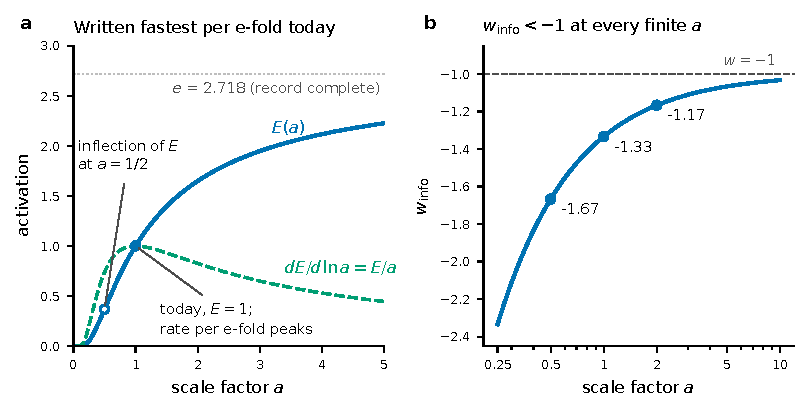
\includegraphics[width=\textwidth]{figures/part1/fig_activation.pdf}
\caption{(a) The activation function $E(a)=\exp(1-1/a)$ (Eq.~\eqref{eq:Ea}) and the record written per e-fold, $dE/d\ln a=E/a$, which peaks at $a=1$; $E$ has its inflection at $a=1/2$ and tends to $e$. (b) The equation of state of the record term, $w_{\rm info}=-1-1/(3a)$: $-1.67$, $-1.33$ and $-1.17$ at $a=0.5$, 1 and 2. \derived}\label{fig:activation}
\end{figure}
The decoherence constraint requires the informational energy density to satisfy
\begin{equation}
\dot\rho_{\rm info}=\rho_{\rm info}\,\frac{H}{a}. \label{eq:law_constraint}
\end{equation}
\conjecture\ (the record constraint, a premise). With $\dot a=aH$ this is $d\ln\rho_{\rm info}/da=1/a^2$, a separable equation that integrates directly. The
integral must start at $a=1$, because $\int_0^ada'/a'^2$ diverges; normalized to today,
\begin{equation}
\ln\frac{\rho_{\rm info}(a)}{\rho_{\rm info}(1)}=\int_1^a\frac{da'}{a'^2}=1-\frac1a,\qquad
E(a)\equiv\frac{\rho_{\rm info}(a)}{\rho_{\rm info}(1)}=\exp\!\left(1-\frac1a\right)=e^{-z}. \label{eq:Ea}
\end{equation}
\derived\ given Eq.~\eqref{eq:law_constraint}. The normalization $E(1)=1$ is set by definition. The properties of $E(a)$ follow directly:
\begin{itemize}
\item $E(a)\to0$ as $a\to0$: no record cost before stable massive particles exist.
\item $E(1)=1$: normalization today.
\item $dE/da=E/a^2>0$ always: each decoherence event is irreversible. The ledger only grows.
\item $E(\infty)=e\approx2.718$: the accumulated cost approaches a finite value without arriving. The universe matures rather than tears apart.
\item $E(z)=\exp(-z)$: pure exponential decay with redshift --- the simplest form for a quantity growing from zero at early times to a finite value
today. $E$ reaches 10, 50 and 90\,\% of today's value at $z=2.30$, $0.69$ and $0.11$; at recombination ($a\approx10^{-3}$) it is $\exp(-999)$, zero for every
purpose \calc.
\item $d^2E/da^2=E(1-2a)/a^4$ vanishes at $a=1/2$ (the inflection, $z=1$), and the record written per e-fold, $dE/d\ln a=E/a$, is largest at $a=1$ \derived.
\end{itemize}
The $1/a$ in the exponent has a physical reading: $E(a)$ is the exponential of the cumulative information surface density on the cosmic horizon. On this
reading what drives the record term is not how much total information the universe has produced, but how densely that information is packed on the
horizon surface \interp.

\subsection{The variational formulation}\label{sec:law_variational}
The thermodynamic result admits a variational formulation, connecting IAM's Law to standard field-theoretic language. Define the scalar
\begin{equation}
\phi(t)\equiv\ln E(a)=1-\frac1a , \label{eq:law_phi}
\end{equation}
which satisfies the decoherence constraint $\dot\phi=\dot a/a^2=H/a$. This is not a Klein--Gordon equation. $\phi$ does not propagate independently; it
tracks the cumulative decoherence history. The informational action is
\begin{equation}
S_{\rm info}=\int\left[-\frac{3H_0^2}{8\pi G}\beta_me^{\phi}+\lambda\left(\dot\phi-\frac{H}{a}\right)\right]\sqrt{-g}\,d^4x, \label{eq:law_action}
\end{equation}
where $\lambda$ is a Lagrange multiplier enforcing the decoherence constraint. Variation with respect to the metric returns Eq.~\eqref{eq:Hm}. Written out
in the FRW minisuperspace, with lapse $N$, $ds^2=-N^2dt^2+a^2d\mathbf x^2$, $\sqrt{-g}=Na^3$, $\dot\phi\to\phi'/N$, $H\to a'/(Na)$ (primes $d/dt$) and
$\rho_0=3H_0^2/8\pi G$, the Lagrangian per unit comoving volume of gravity, $\Lambda$, matter and the record sector is
\begin{equation}
L=-\frac{3}{8\pi G}\frac{aa'^2}{N}-Na^3\Big(\frac{\rho_{m0}}{a^3}+\rho_\Lambda+\rho_0\beta_me^{\phi}\Big)+\lambda a^3\Big(\phi'-\frac{a'}{a^2}\Big).
\label{eq:law_L}
\end{equation}
The constraint term does not contain $N$: the lapse cancels between $\sqrt{-g}$ and the two time derivatives.
\begin{enumerate}
\item Varying $N$ (then $N=1$): $H^2=\tfrac{8\pi G}{3}\big(\rho_m+\rho_\Lambda+\rho_0\beta_me^{\phi}\big)$, which is Eq.~\eqref{eq:Hm}; $\lambda$ does not enter.
\item Varying $\lambda$: $\phi'=a'/a^2=H/a$, the constraint, with solution $\phi=1-1/a$.
\item Varying $\phi$: $d(\lambda a^3)/dt=-a^3\rho_0\beta_me^{\phi}$, an equation for the multiplier.
\item Varying $a$, and using 2 and 3: the multiplier terms cancel and the record sector contributes a pressure $P_{\rm info}=-\rho_{\rm info}-\rho_{\rm info}/(3a)$.
\end{enumerate}
\derived\ in the minisuperspace, given the action. The equation of state of the informational energy density follows equally from the continuity equation
$\dot\rho+3H(\rho+P)=0$ with $d\ln\rho_{\rm info}/d\ln a=1/a$:
\begin{equation}
w_{\rm info}(a)=-1-\frac{1}{3a}:\qquad -1.67\ (a=0.5),\quad -1.33\ (a=1),\quad -1.17\ (a=2). \label{eq:law_winfo}
\end{equation}
\derived\ This is a mildly phantom equation of state ($w<-1$) at all finite $a$, approaching $-1$ as $a\to\infty$. The phantom behaviour reflects the
continuous conversion of gravitational binding energy into informational entropy, not a violation of the null energy condition, because $\phi$ is a
thermodynamic variable constrained by geometry, not a propagating field \interp. $w_{\rm info}(a)$ is a formal thermodynamic parametrization of the entropy
completion; it is not a homogeneous dark-energy fluid implemented in the Boltzmann equations. The operational implementation of IAM in observable cosmology
is through the effective matter-sector friction history of Section~\ref{sec:perturbations}, not through a literal new background source term.
Energy--momentum is conserved identically, $\nabla_\mu T^{\mu\nu}_{\rm total}=0$: steps~1 and~4 together are energy conservation for the record sector, which
the Euler--Lagrange equations of a time-reparametrization-invariant action satisfy identically \derived. The constraint $\dot\phi=H/a$ is the record
constraint written as a field equation, so the action assumes the activation function it returns \conjecture; and $H/a$ is not a spacetime scalar, so the
action is defined on the FRW minisuperspace, and writing a covariant form is the next step \openprob.

\subsection{The virial theorem as balance sheet}\label{sec:law_coupling}
IAM's Law says that each record carries a cost. The virial theorem tells you how much energy crosses the record boundary at each virialization event.
Together they give the cosmological coupling constant with no free parameter. For a self-gravitating system in virial equilibrium, half the gravitational
binding energy goes into the geometric channel (spacetime curvature, standard general relativity) and half into the informational channel (the record
cost, paid to the encoding surface). Applied to the whole ensemble of bound structure (Assumption~3), the informational energy density at $a=1$ is
\begin{equation}
\rho_{\rm info}(a{=}1)=\tfrac12\rho_m=\frac{\Omega_m}{2}\,\rho_{\rm crit}. \label{eq:law_rhoinfo1}
\end{equation}
Since $\rho_{\rm info}(1)=\beta_mE(1)\rho_{\rm crit}=\beta_m\rho_{\rm crit}$,
\begin{equation}
\beta_m=\frac{\Omega_m}{2}=0.15765\quad(\Omega_m=0.3153~\text{\cite{Planck2018VI}}). \label{eq:law_beta}
\end{equation}
\prediction\ The $1/2$ partition of the virial theorem is the coupling constant of IAM's Law at cosmological scales. It is not fitted: every IAM
chain carries it at this value (Level~1 and the baryon chain as the MGCAMB amplitude $\mu_0=-0.13495$), and only the four free-$\mu_0$ test chains sample the amplitude (Chapter~\ref{ch:dual}).

\subsection{The dual-sector split}\label{sec:law_dualsector}
IAM's Law applies to matter on timelike worldlines.
\begin{definition}[Decoherence eligibility]
A degree of freedom undergoes gravitational decoherence if and only if it propagates on a timelike worldline ($d\tau>0$).
\end{definition}
Decoherence is a dynamical process requiring a finite proper time interval $\Delta\tau>0$. Photons propagate on null geodesics: $ds^2=0$, $\Delta\tau=0$. A
photon does not accumulate proper time. It does not virialize. It pays no record cost. The null interval is geometry; that the record term then enters the
matter perturbations alone is the sector rule \conjecture.

\textbf{Proposition (dual-sector coupling).} For matter (timelike worldlines), $S_{\rm info}>0$, yielding
\begin{equation}
\mu(a)=\frac{H^2_{\Lambda{\rm CDM}}(a)}{H^2_{\Lambda{\rm CDM}}(a)+\beta_mE(a)H_0^2}<1. \label{eq:mu}
\end{equation}
For photons (null worldlines), $S_{\rm info}=0$, yielding
\begin{equation}
\Sigma(a)=1. \label{eq:law_Sigma}
\end{equation}
At $a=1$, $\mu=1/(1+\beta_m)=0.8638$ and $\mu_0\equiv\mu(z{=}0)-1=-\beta_m/(1+\beta_m)=-0.136$ ($-0.13618$ at $\beta_m=0.15765$), with no free parameter
beyond $\Lambda$CDM \prediction. The change $1-\mu=13.62\,\%$ is the change in the effective coupling for matter today, not the change in growth
(Section~\ref{sec:perturbations}). The $\beta_mE(a)$ term does not modify the background Friedmann equation: the Weyl tensor of exact FRW vanishes, and any
entropy functional sourced by inhomogeneous structure formation must vanish in this limit. The modification operates at the perturbation level, entering
through the effective Hubble friction for matter perturbations while leaving the background and photon sector unchanged.

\section{Perturbations: why growth is weaker and light is not}\label{sec:perturbations}
The entropy completion of Section~\ref{sec:law_global} is a formal thermodynamic statement. This section shows how it enters observable cosmology: not as
a universal homogeneous background modification, but through the timelike matter-sector perturbation equations. The background FRW expansion rate, photon
geodesics, CMB power spectra, BAO positions and lensing are unchanged. The sole observable effect is suppressed matter growth through enhanced Hubble
friction in the matter growth equation.

\subsection{The informational field does not fluctuate}
The scalar $\phi=1-1/a$ is defined through the background apparent horizon radius $\tilde r_A=c/H(t)$ and therefore depends only on the homogeneous
expansion rate $H(t)$. In linear scalar perturbation theory, local overdensities $\delta\rho$ source the metric potentials $\Psi$ and $\Phi$, but they do not
shift the background-defined apparent horizon at first order. Therefore
\begin{equation}
\delta\phi=0 \label{eq:law_dphi}
\end{equation}
in linear perturbation theory. This is analogous to the cosmological constant, which satisfies $\delta\Lambda=0$: both are properties of the spacetime
geometry, not of the local matter content. Formally, perturbing the constrained action, Eq.~\eqref{eq:law_action}: variation with respect to $\lambda$ gives
the perturbed constraint $\delta\dot\phi=0$, and with the initial condition $\delta\phi(a_i)=0$ the field remains unperturbed at all times. This is a
property of the reduced action, in which $\phi$ has no spatial dependence \conjecture.

\subsection{Standard perturbations with modified matter-sector friction}
With $\delta\phi=0$ the cosmological perturbation equations are those of general relativity. The sole effect of the entropy completion is an additional
contribution to the effective matter-sector expansion rate $H_m$ of Eq.~\eqref{eq:Hm}, which enters only the matter growth equation as enhanced Hubble
friction. The background FRW expansion rate is unchanged. In conformal Newtonian gauge~\cite{MaBertschinger1995},
$ds^2=a^2[-(1+2\Psi)d\tau^2+(1-2\Phi)d\mathbf x^2]$, on sub-horizon scales:
\begin{align}
&\text{Poisson equation:} && k^2\Psi=-4\pi Ga^2\rho_m\delta_m, \label{eq:law_poisson}\\
&\text{no anisotropic stress:} && \Psi=\Phi, \label{eq:law_noaniso}\\
&\text{matter growth:} && \ddot\delta_m+2H_m\dot\delta_m-4\pi G\rho_m\delta_m=0, \label{eq:law_growth}
\end{align}
since $\delta\phi=0$ introduces no anisotropic stress from the informational sector. These are the general-relativistic perturbation equations; the only
modification from $\Lambda$CDM is the enhanced friction term $2H_m\dot\delta_m$, which suppresses matter growth. This is the mechanism of $\mu(a)<1$.

\subsection{$\mu(a)$ and $\Sigma(a)$ as ratios of Hubble rates}
Mapping to the $\mu$--$\Sigma$ framework: if matter perturbations see $H_m$ in the density parameter that sources their growth,
$\Omega_m^{(m)}(a)=8\pi G\rho_m/(3H_m^2)=\Omega_m(a)\,H^2/H_m^2$, the effective gravitational coupling for matter perturbations is the ratio of Hubble rates
squared,
\begin{equation}
\mu(a)=\frac{E^2_{\Lambda{\rm CDM}}(a)}{E^2_{{\rm eff},m}(a)}=\frac{H^2_{\Lambda{\rm CDM}}(a)}{H^2_{\Lambda{\rm CDM}}(a)+\beta_mE(a)H_0^2}<1, \label{eq:law_muratio}
\end{equation}
where $E_{\Lambda{\rm CDM}}=H/H_0$ is the dimensionless expansion rate (not the activation function). This is a mapping onto the $\mu$--$\Sigma$ form; deriving the form is the next step \interp. The suppression $\mu<1$ arises because the enhanced friction reduces the effective matter density parameter,
$\Omega_m^{(m)}(a)<\Omega_m(a)$, so matter clusters less effectively than in $\Lambda$CDM. Values (Planck 2018 background, $\beta_m=0.15765$):

\begin{center}
\begin{tabular}{lcccccccc}\hline
$z$ & 0 & 0.2 & 0.3 & 0.5 & 0.7 & 1 & 2 & 3\\\hline
$\mu$ & 0.8638 & 0.9050 & 0.9218 & 0.9482 & 0.9661 & 0.9822 & 0.9977 & 0.9996\\
$H_m/H$ & 1.0759 & 1.0512 & 1.0415 & 1.0270 & 1.0174 & 1.0090 & 1.0012 & 1.0002\\\hline
\end{tabular}
\end{center}
\calc\ with $\mu\to1$ at high redshift as $E(a)\to0$ (Fig.~\ref{fig:law_derivations}b).

The friction form, Eq.~\eqref{eq:law_growth}, and the coupling form, Eq.~\eqref{eq:law_muratio}, are two implementations of the same term, and they do not give
the same growth. With $D'=dD/d\ln a$ and the same early amplitude:
\begin{align}
\text{(i) }G_{\rm eff}=\mu G:&\quad D''+\Big(2+\frac{d\ln H}{d\ln a}\Big)D'-\tfrac32\Omega_m(a)\,\mu\,D=0,\\
\text{(ii) friction, }\Lambda\text{CDM clock:}&\quad D''+\Big(\frac{d\ln H}{d\ln a}+2\frac{H_m}{H}\Big)D'-\tfrac32\Omega_m(a)D=0,\\
\text{(iii) whole equation on }H_m:&\quad D''+\Big(2+\frac{d\ln H_m}{d\ln a}\Big)D'-\tfrac32\frac{\Omega_ma^{-3}H_0^2}{H_m^2}D=0 .
\end{align}
Form (ii) is Eq.~\eqref{eq:law_growth} written with $\dot\delta=HD'$. Today $\Delta D/D=-0.78\,\%$ (i, the Level~1 form), $-0.67\,\%$ (ii, the Level~2 form) and
$-1.87\,\%$ (iii) \calc. Which implementation the record term implies is an open problem \openprob; every growth number in this book names its form. In form (i)
$f\sigma_8$ is lower than in $\Lambda$CDM by $4.25\,\%$, $2.17\,\%$, $1.35\,\%$ and $0.41\,\%$ at $z=0$, $0.3$, $0.5$ and $1$ \calc.

Since both potentials satisfy the unmodified Poisson equation, Eq.~\eqref{eq:law_poisson}, with no anisotropic stress, Eq.~\eqref{eq:law_noaniso}, photon
geodesics are determined by $(\Psi+\Phi)/2=\Psi$ without modification. Therefore $\Sigma(a)=1$. The photon exemption at the perturbation level is a
consequence of $\delta\phi=0$ --- that $\phi$ is a horizon quantity, not a local field. CMB power spectra, CMB lensing, BAO angular positions and supernova
luminosity distances are unchanged; IAM and $\Lambda$CDM produce CMB TT spectra differing by less than $0.13\,\%$ at $\ell>30$ (Chapter~\ref{ch:theory}; the comparison is drawn by \texttt{tests/\allowbreak{}iam\_camb\_full\_boltzmann.py}, and the spectra themselves are not stored in the repository) \calc.

\subsection{Where this sits among modified-growth models}
Most modified-gravity theories predict $\mu>1$ (enhanced growth) or correlated deviations in both $\mu$ and $\Sigma$. $f(R)$ gives $\mu>1$ with
$\Sigma=1$~\cite{PogosianSilvestri2008}; the normal branch of DGP gives $\mu>1$ with $\Sigma=1$~\cite{DGP2000,KoyamaMaartens2006}; in Horndeski
theories~\cite{Horndeski1974} $\mu-1$ and $\Sigma-1$ of opposite sign are strongly disfavoured~\cite{PogosianSilvestri2016}. The self-accelerating branch of
DGP gives $\mu<1$ with $\Sigma=1$, the same sign as IAM, but it carries a ghost~\cite{Koyama2007} and is in strong tension with growth and distance
data~\cite{Fang2008}. The IAM signature --- weakened matter growth with unmodified lensing --- is characteristic of a model that modifies matter-sector dynamics
through Hubble friction without introducing anisotropic stress or touching photon geodesics, and with no new propagating field. It is an unusual
combination \observed.

\subsection{Numerical validation}
Level~1 validation used MGCAMB~\cite{Zhao2009MGCAMB,Wang2023MGCAMB} with Cobaya~\cite{Torrado2021} in the $\mu$--$\Sigma$ parametrization: twelve chains, four
dataset combinations (Planck alone, Planck with redshift-space distortions, Planck with BAO, Planck with Pantheon+~\cite{Brout2022}). Level~2 validation used
a direct modification of CAMB~\cite{Lewis2000CAMB} implementing the matter growth equation, Eq.~\eqref{eq:law_growth}, through the matter-sector expansion rate
in the Boltzmann solver (three chains). Two Level~2b exploratory runs applying the modification at the background Friedmann level produced
$H_0\approx61.5$\,km\,s$^{-1}$Mpc$^{-1}$, which BAO and the distance ladder exclude: the term belongs in the perturbations. Every chain ends at
$R-1\le0.010$~\cite{Gelman1992} with no discarded run (Chapter~\ref{ch:dual}) \measured.

\section{The exponent: from the horizon and from the halos}\label{sec:law_exponent}
\subsection{Top-down: from horizon thermodynamic consistency}
The top-down derivation requires the cumulative informational entropy to reproduce $E(a)=\exp(1-1/a)$. Per unit $\ln a$, Eqs.~\eqref{eq:rate}--\eqref{eq:Sdot}
give $dS_{\rm info}/d\ln a=(dS_{\rm info}/dt)/H\propto\rho_mD^nf/(T_HA_H)$ (the $H$ in $\dot I$ cancels the $1/H$). Under matter-domination scalings,
$H\propto a^{-3/2}$, $A_H\propto a^3$, $T_H\propto a^{-3/2}$, $D\propto a$, $f=1$:
\begin{equation}
\frac{dS_{\rm info}}{d\ln a}\propto\frac{\rho_m\,D^n f}{T_H\,A_H}\propto\frac{a^{-3}a^n}{a^{-3/2}a^3}=a^{\,n-9/2}. \label{eq:law_dSdlna}
\end{equation}
Converting to $da$, $dS_{\rm info}/da\propto a^{\,n-11/2}$, and integrating,
\begin{equation}
S_{\rm info}(a)\propto\frac{a^{\,n-9/2}}{n-9/2}. \label{eq:law_Sa}
\end{equation}
For $S_{\rm info}(a)\propto-1/a+{\rm const}$, the form required by $E(a)=\exp(1-1/a)$, we need $a^{\,n-9/2}=a^{-1}$:
\begin{equation}
n-\frac92=-1\quad\Longrightarrow\quad n=\frac72 . \label{eq:law_n}
\end{equation}
\calc\ given the rate law. The same condition in the form ``the record surface density $D/A_H$ falls as $a^{-2}$'': the remaining factor
$\rho_mD^{n-1}f/(T_Ha)\propto a^{\,n-7/2}$ is constant only for $n=7/2$; the two statements are one. Integrating Eqs.~\eqref{eq:rate}--\eqref{eq:Sdot} with the
full $\Lambda$CDM growth factor gives $dS_{\rm info}/d\ln a\propto a^{-1.02}$ for $n=7/2$ over $0.01\le a\le0.1$ (and $a^{-2.02}$, $a^{-1.52}$, $a^{-0.53}$ for
$n=5/2$, $3$, $4$); the $\Lambda$ era steepens it, to $a^{-1.57}$ over $0.25\le a\le1$ for $n=7/2$ (Fig.~\ref{fig:law_derivations}a) \calc. The scaling fixes the
shape of the history, not its amplitude: the coefficient of $1/a$ is the normalization of $S_{\rm info}$ \openprob.

\begin{figure}[htbp]\centering
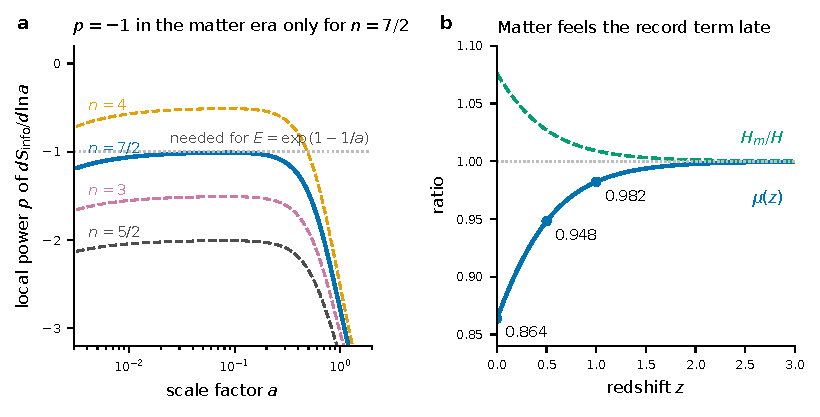
\includegraphics[width=\textwidth]{figures/part1/fig_law_derivations.pdf}
\caption{(a) The local power $p=d\ln(dS_{\rm info}/d\ln a)/d\ln a$ for the rate law $\dot I\propto\rho_mD^nfH$ accumulated per unit horizon area at the horizon
temperature (Eqs.~\eqref{eq:rate}--\eqref{eq:Sdot}), full $\Lambda$CDM growth ($\Omega_m=0.3153$, $\Omega_r=9.1\times10^{-5}$). $E(a)=\exp(1-1/a)$ needs $p=-1$
(dotted). Fitted over $0.01\le a\le0.1$: $-2.02$, $-1.52$, $-1.02$, $-0.53$ for $n=5/2$, $3$, $7/2$, $4$ \calc. (b) $\mu(z)=H^2/(H^2+\beta_mE(a)H_0^2)$ and $H_m/H$
for $\beta_m=0.15765$: $\mu=0.864$, $0.948$, $0.982$ at $z=0$, $0.5$, $1$ \calc. Script: \texttt{docs/book/figscripts/\allowbreak{}fig\_p1\_law\_derivations.py}.}\label{fig:law_derivations}
\end{figure}

\subsection{Bottom-up: from structure formation}
The bottom-up route integrates IAM's Law over the halo mass function~\cite{PressSchechter1974}. The rate of information production per virialization event
is set by the record cost at the virialization boundary (the local expression of IAM's Law): the energy a bound structure writes is its kinetic half,
$K\approx\tfrac12|W|$. In the Press--Schechter description the peak height of a halo of mass $M$ is $\nu=\delta_c/[\sigma(M)D(a)]$, so $\nu\propto D^{-1}$ at fixed
mass \derived. Summing the virial kinetic energy over all halos with measured mass functions, $n_{\rm eff}=d\ln[(dU/d\ln a)/f]/d\ln D$ is not constant: it
runs from about $5.5$ at $z=9$ through $7/2$ at $z\approx3$--$4$ to about $2$ at $z=1$, and averages $3.9$--$4.3$ over the matter-dominated window
$z=2.3$--$9$ for Press--Schechter, Sheth--Tormen and Tinker et al.\ mass functions~\cite{PressSchechter1974,ShethTormen1999,Tinker2008}
(Chapter~\ref{ch:quantumrecords}) \calc. The two directions meet at $7/2$ to within that running; they are not an exact identity, and obtaining a constant $7/2$ from the halos is open \openprob.

\section{The nine-step causal chain}
This section traces the causal sequence by which IAM's Law, applied to gravitational structure formation, produces the observable consequences derived in
Sections~\ref{sec:law_global} and~\ref{sec:perturbations}. Steps 1--5 follow from established physics; the references are to the standard results used at
each stage.
\begin{enumerate}
\item Gravitational interaction. Matter interacts gravitationally, initiating collapse of overdense regions (general relativity~\cite{Einstein1915}).
\item Gravitational collapse. Matter clusters into bound systems: halos, galaxies, stars (structure formation~\cite{PressSchechter1974}).
\item Quantum decoherence. Gravitational interaction resolves quantum superpositions into definite classical states (Eq.~\eqref{eq:law_entangle},
\cite{Zurek2003}).
\item Irreversible information production. Each decoherence event produces classical information ($I=\log_2N$ bits, Eq.~\eqref{eq:law_bits}) that cannot be
recovered.
\item Landauer cost. Information production carries an irreducible energy cost of $k_BT_H\ln2$ per bit at the horizon temperature (IAM's Law,
Eq.~\eqref{eq:law}).
\item Holographic encoding. The produced information is bounded by and encoded on the cosmic horizon area~\cite{Bekenstein1973,tHooft1993,Susskind1995},
contributing $S_{\rm info}$ to the entropy functional \conjecture.
\item Informational term. The modified first law $-dE=T_H\,d(S_{\rm geo}+S_{\rm info})$ introduces the additional term $\beta_mE(a)H_0^2$ in the matter-sector
perturbation equations (Eq.~\eqref{eq:Hm}) \conjecture.
\item Modified growth. The matter-sector perturbation equations acquire enhanced Hubble friction, suppressing growth: $\mu(a)=H^2_{\Lambda{\rm CDM}}/H_m^2<1$.
\item Feedback suppression. Suppressed growth lowers the effective matter density parameter seen by perturbations, weakening gravitational collapse and
reducing the amplitude of subsequent decoherence events \conjecture.
\end{enumerate}
Step 9 feeds back into step 1 with reduced amplitude, and the chain self-regulates. Gravity appears at two points in the chain: as the initiating cause of
decoherence (step 1) and as the observable modified by the resulting informational term (step 8). The finite limit $E(a)\to e$ is a property of the
function of Eq.~\eqref{eq:Ea}; reading it as the outcome of this feedback is interpretation, taken up with the rest of the chain in
Chapter~\ref{ch:theoryinterp} \interp.

\section{Black holes: the local saturation limit}\label{sec:law_blackholes}
Sections~\ref{sec:law_local}--\ref{sec:perturbations} address the distributed regime of IAM's Law: structure formation producing decoherence events across
many halos, encoding cumulatively on the growing cosmic horizon. This section addresses the concentrated local limit: what IAM's Law gives when the local
information production saturates the encoding capacity of the nearest bounding surface. The result is the standard black-hole formation condition, read
here from the informational saturation criterion rather than from gravitational collapse directly.

\subsection{The holographic saturation condition}
A black hole forms when the informational entropy from gravitational decoherence within radius $R$ saturates the Bekenstein--Hawking bound on the bounding
surface:
\begin{equation}
\frac{S_{\rm info}(R)}{A(R)}\ge\frac{k_B}{4\ell_P^2}. \label{eq:law_saturation}
\end{equation}
Setting $S_{\rm info}=S_{\rm BH}=4\pi Gk_BM^2/(\hbar c)$ at the Schwarzschild radius $r_s=2GM/c^2$:
\begin{equation}
\frac{4\pi Gk_BM^2/(\hbar c)}{4\pi\cdot4G^2M^2/c^4}=\frac{k_Bc^3}{4\hbar G}=\frac{k_B}{4\ell_P^2}. \label{eq:law_hoop}
\end{equation}
\derived\ The holographic bound is exactly saturated at the Schwarzschild radius. Read this way, Eq.~\eqref{eq:law_saturation} is the Thorne hoop
conjecture~\cite{Thorne1972} in informational language: the hoop conjecture is the holographic bound in geometric language \interp\ (Chapter~\ref{ch:blackholes}).

\subsection{The two-horizon framework}
Both the black-hole horizon, at $T_{\rm BH}=\hbar c^3/(8\pi GMk_B)$, and the cosmic horizon, at $T_H=\hbar H/(2\pi k_B)$~\cite{GibbonsHawking1977}, are thermal
encoding surfaces. Setting $T_{\rm BH}=T_H$ gives the thermal equilibrium mass
\begin{equation}
M_{\rm eq}=\frac{c^3}{4GH}, \label{eq:law_Meq}
\end{equation}
and $T_{\rm BH}/T_H=M_{\rm eq}/M$ \derived. At the present epoch $M_{\rm eq}=2.33\times10^{22}\,M_\odot$ ($H_0=67.16$; $2.32\times10^{22}$ at $67.4$) \calc ---
far exceeding the largest known black hole. All astrophysical black holes satisfy $T_{\rm BH}\gg T_H$: information flows from hot local horizons to the cold
cosmic horizon, at the black-body Hawking rate
\begin{equation}
\Gamma=\frac{P}{k_BT_{\rm BH}\ln2}=\frac{c^3}{1920\,GM\ln2}\ \text{bits\,s}^{-1},\qquad P=\frac{\hbar c^6}{15360\pi G^2M^2}, \label{eq:law_Gamma}
\end{equation}
$152.5$ bits\,s$^{-1}$ for one solar mass \calc\ (greybody factors change the coefficient~\cite{Page1976}). The cosmic horizon is the final repository;
all locally encoded information migrates to the global ledger \interp.

\subsection{Black holes as preferred early-universe encoding surfaces}
The activation function $E(a)=\exp(1-1/a)$ tracks the encoding transition. At early times ($a\ll1$), the cosmic horizon is small and the Gibbons--Hawking
temperature is high, making cosmic-horizon encoding inefficient. Information from early gravitational decoherence is encoded primarily on local black-hole
horizons. As the universe expands, large-scale structure formation produces distributed decoherence, and the cosmic horizon grows and cools, eventually
dominating as the encoding surface. The activation function is the quantitative record of this transition. This suggests a natural thermodynamic context
for the massive black holes observed at high redshift: in the early universe, before the cosmic horizon grows large enough to encode
efficiently, black holes are the nearest available encoding surfaces. Within the IAM framework this is a consequence of the saturation condition rather
than an anomaly requiring separate explanation \interp\ (Chapter~\ref{ch:theoryinterp}).

\section{The thermodynamic arrow of time and the coincidence problem}\label{sec:law_arrow}
IAM's Law is irreversible by construction: each Landauer cost payment is permanent, and $S_{\rm info}$ can only grow. This section records two consequences
of that irreversibility that are not independent predictions but structural properties of the activation function $E(a)$ already derived.

The activation function $E(a)=\exp(1-1/a)$ is monotonically increasing in $a$. Since decoherence events are irreversible and Landauer costs are permanent,
$E(a)$ cannot decrease. Expressed in redshift, $E(z)=\exp(-z)$ (Eq.~\eqref{eq:Ea}). The thermodynamic arrow of time follows directly: the informational
content of the universe increases monotonically with cosmic time. At recombination ($a\approx10^{-3}$) $E(a)\approx0$; at the present epoch $E(1)=1$; at late
times $E(a)\to e$. The arrow is not an additional assumption. It is a property of $E(a)$ inherited from the irreversibility of decoherence encoded in IAM's
Law \interp\ (Chapter~\ref{ch:time}).

The coincidence problem --- why the informational energy density $\rho_{\rm info}\propto E(a)$ becomes important at approximately the same epoch as
structure formation peaks --- has a direct causal explanation within IAM. The informational term $\beta_mE(a)$ is sourced by structure formation. It grows
when structure formation is active and self-regulates as suppressed growth reduces the decoherence rate. The coincidence between dark-energy domination
and the peak of structure formation is therefore, on this reading, a consequence of IAM's Law rather than a free parameter: the same process drives both
\conjecture\ (Chapter~\ref{ch:theoryinterp}).

\section{Observational consistency}
\subsection{The primary test: $\beta_m=\Omega_m/2$}
The primary quantitative test of IAM's Law at cosmological scales is the coupling constant $\beta_m=\Omega_m/2=0.15765$, fixed by the virial theorem with no
free parameter. Seventeen MCMC chains were run with Cobaya~\cite{Torrado2021} against the Planck likelihoods --- the Planck 2018 low-$\ell$ TT and EE and lensing~\cite{Planck2018V,Planck2018VIII}, with the Planck 2018 \texttt{plik\_lite} TT, TE, EE at high $\ell$ for Level~1 and the PR4 NPIPE CamSpec TT, TE, EE~\cite{Rosenberg2022} for Level~2: twelve with MGCAMB~\cite{Hojjati2011} (Level~1), three with the modified CAMB (Level~2) and two Level~2b diagnostics; with the baryon chain below, eighteen in all. All converged to $R-1\le0.010$
with no discarded runs, no parameter adjustments and no excluded redshift ranges. The coupling is not a fitted parameter of these chains. Of the eighteen, nine carry it fixed at the prediction (Level~2 and 2b as
$\beta_m=0.15765$; Level~1 and the baryon chain as the MGCAMB amplitude $\mu_0=-0.13495$), five are the $\Lambda$CDM controls and four sample $\mu_0$ freely as a test; the test is whether the fixed coupling is consistent with Planck. It is (Table~\ref{tab:law_consistency}; Chapter~\ref{ch:dual}).

\begin{table}[htbp]\centering
\caption{Quantitative consistency checks. Every IAM chain carries the coupling fixed at $\beta_m=\Omega_m/2$ (Level~1 as $\mu_0=-0.13495$); only the four free-$\mu_0$ test chains sample it. $\Delta\chi^2$ is the difference of the lowest $\chi^2$ in each chain after the 30\,\% burn-in, same data, same code. Chain values are from the
final chain files (Chapter~\ref{ch:dual}) \measured; distances in $\sigma$ \calc.}\label{tab:law_consistency}
\begin{tabularx}{\linewidth}{>{\raggedright\arraybackslash}Xll}
\hline
Quantity & IAM & Result\\\hline
$\beta_m$ & $\Omega_m/2=0.15765$, fixed & fixed at the prediction in every IAM chain\\
$\Delta\chi^2$ vs $\Lambda$CDM, Level 2 & no added parameter & $+0.54$\\
$\Delta\chi^2$, Level 1 (four combinations) & no added parameter & $+0.56$ to $+1.73$\\
$\sigma_8$ & suppressed & $0.809\to0.800$ (Level 2)\\
$H_0$, light & unchanged & $67.16\pm0.47$; $-0.37\sigma$ from Planck $67.36\pm0.54$\\
$H_0$, matter & $67.16\sqrt{1+\beta_m}$ & $72.26$; $-0.75\sigma$ from SH0ES $73.04\pm1.04$~\cite{Riess2022}\\
free $\mu_0$ (Level 1) & prediction $-0.136$ & 90\,\% interval contains the prediction and $0$\\\hline
\end{tabularx}
\end{table}
IAM's own equations, with the coupling fixed and no added parameter, reproduce the Planck data as well as $\Lambda$CDM does: $\Delta\chi^2=+0.54$.

\subsection{The sector-dependent Hubble split}
The sector-dependent Hubble split $H_0^{(\rm matter)}/H_0^{(\rm photon)}=\sqrt{1+\beta_m}=1.076$ is a direct consequence of the dual-sector coupling: at $a=1$,
$H_m^2=H_0^2(1+\beta_m)$ \derived. The two values are not a tension. They are measurements of two distinct physical quantities --- light-based probes read
$H_0$, probes of the matter flow read $H_0\sqrt{1+\beta_m}$ --- and both come from a single posterior with no free parameter beyond $\Lambda$CDM:
$67.16\to72.26$\,km\,s$^{-1}$Mpc$^{-1}$ \calc.

Gravitational-wave standard sirens provide an independent test. Binary neutron-star mergers occur in galaxies --- matter-sector objects --- so their host
galaxy recession velocities probe the matter-sector Hubble flow. IAM predicts
\begin{equation}
H_0^{\rm sirens}=H_0^{\rm CMB}\sqrt{1+\beta_m}=67.16\times1.0759=72.26\ \text{km\,s}^{-1}\text{Mpc}^{-1}. \label{eq:law_sirens}
\end{equation}
\prediction\ With one event so far, analyses of GW170817 range from $70.0^{+12.0}_{-8.0}$~\cite{Abbott2017Siren} and $68.9^{+4.7}_{-4.6}$~\cite{Hotokezaka2019} to
$75.46^{+5.34}_{-5.39}$~\cite{Palmese2024}\,km\,s$^{-1}$Mpc$^{-1}$; one event is not yet precise enough to separate the two values \observed; tens of sirens will separate them.

\subsection{Measuring $\mu_0=-0.136$}
IAM's Law gives $\mu_0=-0.136$ with no free parameter. The DESI 2024 full-shape analysis~\cite{DESI2024VII} gives $\mu_0=0.11^{+0.45}_{-0.54}$, consistent
with both the prediction and general relativity \observed. The forecast for Euclid, Planck lensing and DESI, made with the IAM $\mu(z)$ itself, is in
Section~\ref{sec:sp_euclid}. Tighter constraints will either
sharpen the agreement or reveal a discrepancy; both outcomes carry information about the entropy-completion identification at the heart of IAM's Law.

\subsection{The cosmological constant and the baryon density}
The results in this subsection are of a different kind from those above. The preceding subsections document IAM's Law producing predictions consistent
with observational data --- a necessary but not sufficient condition for a law. This subsection concerns two numbers that are free parameters of
$\Lambda$CDM, the cosmological constant and the baryon density; within IAM they are tied together by one relation.

\textbf{The cosmological constant.} The observed ratio $\Lambda_{\rm obs}/\rho_{\rm vac}$ has resisted derivation for over fifty years. Within IAM this ratio
is read as the fraction of Planck-area horizon bits written by baryonic decoherence over cosmic history \conjecture. Written in Planck units, the observed
$\rho_\Lambda/\rho_{\rm vac}=(3\Omega_\Lambda/8\pi)(\ell_P/\ell_H)^2$ identically, $1.133\times10^{-123}$ at $H_0=67.4$ and $\Omega_\Lambda=0.6847$~\cite{Planck2018VI} \calc. The
baseline expression of Chapter~\ref{ch:lambda},
\begin{equation}
\frac{\Lambda_{\rm obs}}{\rho_{\rm vac}}=\frac2\pi\Big(\frac{\ell_P}{\ell_H}\Big)^2\frac{\Omega_b}{\Omega_m}, \label{eq:law_ccbase}
\end{equation}
gives $1.380\times10^{-123}$ ($\Omega_b=0.0493$, $\Omega_m=0.3153$), $1.22$ times the measured value \calc. The de Sitter encoding surface, the horizon set by
$\Lambda$ alone, has the Gibbons--Hawking temperature $T_{dS}=T_H\sqrt{\Omega_\Lambda}$, which differs from the Hubble writing temperature by
\begin{equation}
\frac{T_{dS}}{T_H}=\sqrt{\Omega_\Lambda}=\sqrt{0.6847}=0.8275 . \label{eq:law_TdS}
\end{equation}
Applying it, $(2/\pi)(\ell_P/\ell_H)^2\sqrt{\Omega_\Lambda}\,\Omega_b/\Omega_m=1.142\times10^{-123}$, $0.8\,\%$ above the measured ratio for this parameter set
\calc. Set equal to the identity, the corrected expression reduces to the present-epoch relation $\Omega_b/\Omega_m=(3/16)\sqrt{\Omega_\Lambda}$: the
Planck length, the Hubble length and $\pi$ cancel \derived\ (algebra). On the CMB-only chain below it holds to $0.5\,\%$ ($0.7\sigma$) \calc.

\textbf{The baryon asymmetry.} The baryon-to-photon ratio $\eta$ is measured by Big Bang nucleosynthesis~\cite{Cyburt2016} and by the CMB acoustic
peaks~\cite{Planck2018VI}, but not derived from a deeper principle in any existing framework. IAM's Law connects $\eta$ to $\Lambda$ through the
information writing constraint: the cosmological-constant expression contains $\Omega_b$ explicitly. Inverting it --- asking what $\Omega_b$ the observed
$\Lambda$ requires --- constrains $\eta$ through $\eta=273.9\times10^{-10}\,\Omega_bh^2$. A dedicated chain was run with $\Omega_bh^2$ sampled over a flat
range $[0.010,0.040]$, six times wider than the $[0.020,0.025]$ of the other runs, and otherwise as the Level~1 runs (MGCAMB with Cobaya, the full Planck 2018
likelihood, $\mu_0=-0.13495$ fixed). The chain has no access to light-element abundance data; helium is set inside CAMB from $\Omega_bh^2$ by its standard
nucleosynthesis relation. It converged with $R-1=0.009273$ after 22,400 accepted steps:
\begin{equation}
\Omega_bh^2=0.02232\pm0.00014,\qquad \eta=(6.113\pm0.037)\times10^{-10}. \label{eq:law_eta_chain}
\end{equation}
\fitted\ The four Level~1 $\Lambda$CDM chains return the same $\eta$, $6.117$--$6.137\times10^{-10}$: the informational term is off at recombination ($E\to0$), so the chain
checks that the term leaves the early universe intact; it does not test IAM (Chapter~\ref{ch:baryon}).

\textbf{The connection.} The cosmological constant problem and the baryon asymmetry problem are, within IAM, not two independent problems. They are two
expressions of the same information writing constraint: IAM's Law requires a specific baryonic matter density to produce the observed $\Lambda$, and the
Planck CMB likelihood, with no external baryon constraint, returns a density consistent with that requirement. The same $\sqrt{\Omega_\Lambda}$ geometric
correction that closes the cosmological-constant expression also accounts for the offset between the baseline expression and the CMB baryon result,
suggesting a common physical origin within the IAM framework \conjecture. What the data show is one observed present-epoch relation; its derivation --- the
$2/\pi$, the $\sqrt{\Omega_\Lambda}$ and the weighting over cosmic history --- is open (Chapters~\ref{ch:lambda} and~\ref{ch:baryon}) \openprob.

\section{What the law takes from established physics}\label{sec:law_established}
Table~\ref{tab:law_established} lists the established results the chain rests on, so that none of them is mistaken for a new claim. \observed
\begin{table}[htbp]\centering\small
\caption{Established results used by IAM's Law and their role in it.}\label{tab:law_established}
\begin{tabularx}{\textwidth}{@{}>{\raggedright\arraybackslash}p{0.34\textwidth}>{\raggedright\arraybackslash}p{0.27\textwidth}>{\raggedright\arraybackslash}X@{}}\toprule
result & source & role\\\midrule
$S_{\rm BH}=k_BA/4\ell_P^2$ & \cite{Bekenstein1973,Hawking1975} & encoding capacity of a horizon\\
$T_{\rm BH}=\hbar c^3/(8\pi GMk_B)$ & \cite{Hawking1975} & temperature of the surface\\
$E_{\rm bit}\ge k_BT\ln2$ & \cite{Landauer1961,Berut2012,Jun2014} & cost per irreversible bit\\
Einstein equations as an equation of state & \cite{Jacobson1995} & entropy functional $\Rightarrow$ gravity\\
Friedmann equations from the apparent horizon & \cite{CaiKim2005} & extension to cosmology\\
$T_{\rm BH}S_{\rm BH}=\tfrac12Mc^2$ (Schwarzschild) & \cite{Smarr1973,BardeenCarterHawking1973} & the half of the rest energy\\
$\rho_\Lambda/\rho_{\rm vac}\sim(\ell_P/\ell_H)^2$ & \cite{Weinberg1989} & statement of the vacuum-energy problem\\
virial theorem, $2\langle K\rangle+\langle V\rangle=0$ for $1/r$ potentials & \cite{Clausius1870} & the share $\tfrac12$\\
global hypomethylation of cancer cells & \cite{FeinbergVogelstein1983} & direction of the cellular signal\\
Koide relation, $Q=2/3$ & \cite{Koide1982,Koide1983,Koide1983b} & target of the lepton derivation\\
$\mu(a)$, $\Sigma(a)$ parametrization & \cite{PogosianSilvestri2008} & how the law is tested in Boltzmann codes\\\bottomrule
\end{tabularx}
\end{table}
The one new physical identification is in the entropy functional, $S_{\rm total}=S_{\rm geo}+S_{\rm info}$ (Eq.~\eqref{eq:law_Stotal}); everything
else in the cosmology follows from feeding that functional through the Jacobson--Cai--Kim machinery. \conjecture

\section{Assumptions and how the law can fail}\label{sec:assumptions}
Any statement of a law must be explicit about what is assumed and what is derived. The following assumptions underlie IAM's Law and its consequences in
this chapter.

\textbf{Assumption 1 --- gravity is thermodynamic (the Jacobson hypothesis).} The Einstein field equations are an equation of state derivable from the
Clausius relation applied to causal horizons with entropy proportional to area. This hypothesis is supported by the Bekenstein--Hawking
entropy~\cite{Bekenstein1973,Hawking1975}, the Unruh effect~\cite{Unruh1976} and the Cai--Kim derivation of the Friedmann equations from the same
thermodynamic argument~\cite{CaiKim2005}. It is the foundation of Jacobson's 1995 result and is not universally accepted.

\textbf{Assumption 2 --- decoherence-produced information contributes to horizon entropy.} The cost of every irreversible quantum-to-classical transition
in the bulk is encoded on the nearest available encoding surface and contributes to its entropy functional. This is the single new physical identification
introduced by IAM's Law. It is consistent with the holographic principle~\cite{tHooft1993,Susskind1995,Bousso2002} and Landauer's
principle~\cite{Landauer1961}, but has not been independently verified at the level of a complete quantum theory of gravity. This is the same gap that
exists in all thermodynamic approaches to gravity.

\textbf{Assumption 3 --- the virial coupling $\beta_m=\Omega_m/2$ is exact for the ensemble.} The virial theorem in its strict form applies to
systems in stable bound equilibrium. Cosmological structure formation is non-equilibrium. Section~\ref{sec:law_coupling} applies the virial partition to the
ensemble of virialized structures as a whole. The chains show that the consequence is consistent with Planck; whether the coupling is exact is the open question.

\textbf{What is derived, given these} \derived. The activation function $E(a)=\exp(1-1/a)$ from integrating the record constraint
(Section~\ref{sec:law_activation}); the dual-sector split $\mu<1$, $\Sigma=1$ from the null interval of photons ($d\tau=0$) together with the sector rule and
$\delta\phi=0$; the exponent $n=7/2$ from the horizon accounting (Section~\ref{sec:law_exponent}); and $\mu_0=-0.136$ from these inputs with no free
parameter. The record constraint, the rate law and the sector rule are themselves premises \conjecture.

\textbf{Three distinct failure modes.} The assumptions imply three separable levels at which the framework could be falsified, and these levels do not
rise or fall together. Level~1 (core law): Assumption~2 could fail. Decoherence-produced information may not contribute to horizon entropy in the way
identified here; falsification at this level would require a complete theory that explicitly excludes this channel, or a derivation showing the entropy
identification is internally inconsistent. Level~2 (cosmological implementation): the virial coupling of Assumption~3 could fail for the ensemble. A
systematic failure of the perturbation-level growth suppression to fit upcoming survey data would falsify the cosmological model without necessarily
falsifying the core law. Level~3 (broader structural implications): the extensions --- the nine-step chain, the weak force and black holes as encoding surfaces --- are
consequences suggested by the framework but not yet verified at the same level as the core derivation or the cosmological implementation; their failure
would not falsify Level~1 or Level~2.

\section{Discussion}
\subsection{The three-step derivation chain}
\begin{enumerate}
\item Jacobson~\cite{Jacobson1995}: $\delta Q=T\,dS$ on local Rindler horizons, with $S=\eta A$, implies $G_{ab}+\Lambda g_{ab}=8\pi GT_{ab}/c^4$.
\item Cai--Kim~\cite{CaiKim2005}: $-dE=T\,dS_{\rm geo}$ on the FRW apparent horizon, with $S_{\rm geo}=A_H/(4G)$ and $T=H/(2\pi)$, implies
$H^2=(8\pi G/3)\rho+\Lambda/3$.
\item IAM: $-dE=T\,d(S_{\rm geo}+S_{\rm info})$, with $S_{\rm info}$ from gravitational decoherence, implies, for matter, $H_m^2=H^2+\beta_mE(a)H_0^2$.
\end{enumerate}
Step 3 is the only new physical input: gravitational decoherence irreversibly produces classical information, which is holographically encoded on the cosmic
horizon, contributing $S_{\rm info}(a)$ that grows monotonically with cosmic time. Every other element is established physics.

\textbf{What Clausius, Einstein and Jacobson had.} Clausius (1870)~\cite{Clausius1870}: the mechanical face of the virial theorem, $2\langle K\rangle+\langle
V\rangle=0$, derived from Newton's second law. Correct and complete as a mechanical statement; silent on the thermodynamic meaning of $K$. Einstein
(1915)~\cite{Einstein1915}: the geometry of spacetime. Correct and complete as a description of curved geometry; silent on the cost of producing classical
matter. Jacobson (1995)~\cite{Jacobson1995}: gravity as thermodynamics, general relativity derived as an equation of state from $\delta Q=T\,dS$ --- the
machine: specify an entropy, derive a gravity theory. IAM's Law: the missing entropy term is the accumulated cost of classical records; adding it completes
the entropy budget of Jacobson's derivation, and the thermodynamic reading of the virial theorem is the same cost at the local scale \interp.

\subsection{The four fundamental forces}
Gravity and electromagnetism satisfy the virial $1/2$ partition. Gravity: from stellar structure to the cosmological coupling constant, which every
IAM chain carries at the virial value and is consistent with Planck (Section~\ref{sec:law_coupling}). Electromagnetism: for 20 atoms~\cite{ClementiRoetti1974} and 10 molecules at the
Hartree--Fock limit the virial ratio is $1/2$ to machine precision --- an exact verification, because the virial theorem must hold exactly
for converged $1/r$ wavefunctions (Chapter~\ref{ch:virial_law}) \derived. The Chandrasekhar white-dwarf limit, $M_{\rm Ch}=1.456\,M_\odot$ for $\mu_e=2$, is
a consequence of virial equilibrium between electron degeneracy pressure and gravitational collapse~\cite{Chandrasekhar1931} \derived; the strong force
does not enter it. The strong force confines quarks with a linear potential, for which the virial theorem gives the opposite partition,
$2\langle K\rangle=+\langle V\rangle$ (Chapter~\ref{ch:virial_law}): it holds an equilibrium, with the degree of its own potential.

The weak nuclear force does not hold an equilibrium partition. Within IAM this is read as structural rather than coincidental, and the weak force as
excluded by the law's own logic for three independent reasons. First, it violates parity~\cite{Wu1957}: the laws governing weak interactions are not
symmetric under spatial reflection. Second, it violates CP symmetry~\cite{Christenson1964}: it treats matter and antimatter differently, and CP violation is
one of the conditions~\cite{Sakharov1967} for the baryon asymmetry of approximately one excess matter particle per $10^9$ matter--antimatter pairs that
constitutes all observable matter. Third, and most directly: a force whose function is to drive irreversible transitions between stable bound states cannot
simultaneously satisfy an equilibrium condition within them. \conjecture

The weak force is, on this reading, not one of four equals in the IAM framework. It is the precondition for IAM's Law to operate. Without CP violation and
parity violation there is no preferred direction for decoherence, no arrow of time at the particle-physics level, no activation function $E(a)$, and no IAM
sector split. The other three forces maintain equilibrium in the stable structures that decoherence produces. The weak force produces the irreversibility
that makes decoherence possible in the first place. Three forces maintain stable equilibrium structures; one force drives irreversible transitions between
them. IAM's Law governs the boundary between a quantum superposition and a classical record; the weak force is the crossing. That three of the four
forces hold equilibrium structures, and the one exception is the force whose function requires it not to, is structurally consistent with IAM's Law
identifying that boundary as a thermodynamically costly one. Whether this consistency constitutes independent evidence for the law or merely a post-hoc
structural observation is left to the reader \conjecture.

\subsection{Where IAM's Law sits in the landscape of physics}
Every fundamental law in physics describes one side of a boundary. Classical mechanics describes the post-classical regime --- the deterministic evolution
of definite states. General relativity describes the geometry of spacetime --- the curved manifold that results from the distribution of classical matter
and energy. Quantum mechanics describes the pre-classical regime --- the evolution of superpositions before any definite outcome is selected.
Thermodynamics describes the statistical consequences of irreversible processes in the classical regime. The Standard Model describes the fields and
particles that constitute classical matter once it exists.

Each of these frameworks is extraordinarily successful within its tested domain. Each has a gap at the same location: the boundary between quantum
superposition and classical record. Classical mechanics does not explain why the macroscopic world is classical. General relativity does not explain what
it costs to produce the classical matter whose energy curves spacetime. Quantum mechanics describes superpositions but does not provide a mechanism for
why superpositions become definite outcomes. Thermodynamics states that entropy increases but does not derive this from the dynamics of the
quantum-to-classical transition. The Standard Model describes particles but not the process by which quantum fields become particles.

IAM's Law is a statement about the boundary itself. The boundary is the decoherence event: the irreversible transition from quantum superposition to
definite classical outcome described by Eqs.~\eqref{eq:law_entangle}--\eqref{eq:law_rhodiag}. IAM's Law states that this transition carries a thermodynamic
cost (Eq.~\eqref{eq:law}), that this cost is irreversible, and that it is encoded on the nearest available encoding surface. This single statement has the
following consequences, each connecting to an open problem in an established framework \interp:
\begin{itemize}
\item \emph{Classical mechanics.} The macroscopic world is classical because the record cost has been paid. Newton's laws operate in the regime after the
record is written. IAM's Law is the mechanism that produces the regime in which Newton's laws hold.
\item \emph{General relativity.} Jacobson's 1995 derivation~\cite{Jacobson1995} showed that the Einstein equations follow from $\delta Q=T\,dS$ applied to
local causal horizons. The entropy functional was incomplete. IAM's Law identifies the missing term: the accumulated cost of every irreversible
quantum-to-classical transition in the bulk. Adding it closes Jacobson's derivation; the cosmological model of this chapter is the observable consequence.
Beyond completing the entropy functional, IAM's Law reads both of Jacobson's remaining inputs from geometry: $S\propto A$ from causal accessibility, and
$\eta=1/(4\ell_P^2)$ from the ratio $2\pi/8\pi$, with the same ratio setting the minimum horizon area of $4\ell_P^2$ per unit of entropy
(Section~\ref{sec:law_global}). Jacobson's machine --- specify an entropy functional, derive a gravity theory --- then specifies its own entropy functional
from the same causal geometry.
\item \emph{Thermodynamics.} The second law states that entropy increases but does not derive this from the dynamics of the quantum-to-classical
transition. IAM's Law provides the mechanism: entropy increases because every crossing from superposition to record pays an irreversible cost to the
nearest encoding surface. The second law is, on this reading, a corollary. The activation function, monotonically increasing and bounded above, is the
quantitative record of this irreversibility applied across cosmic time.
\item \emph{Quantum mechanics.} The measurement problem --- how quantum superpositions become definite classical outcomes --- is reframed by IAM's Law from a
foundational mystery into a thermodynamic transaction. The transition occurs when a quantum system interacts irreversibly with its environment, producing
classical information at cost $k_BT_H\ln2$ per bit. The transition is not instantaneous collapse but the irreversible orthogonalization of environmental
states described by Eq.~\eqref{eq:law_entangle}. IAM's Law identifies the thermodynamic cost of the transition and shows that this cost, accumulated over cosmic history, has observable cosmological consequences, consistent with current data (Table~\ref{tab:law_consistency}; Chapter~\ref{ch:measurement}); the measurement problem at the level of a complete quantum theory of gravity remains open.
\item \emph{The cosmological constant.} The vacuum baseline of information production --- quantum vacuum fluctuations producing a constant,
epoch-independent rate of classical information --- maps to $\Lambda$ through the Jacobson mechanism. The cosmological constant is, on this reading, the
encoding cost of the vacuum baseline. The structural term $\beta_mE(a)$ is the encoding cost of gravitational structure formation above that baseline.
IAM's Law places both terms in the same entropy budget, unified by the same cost per bit. The quantitative consequence is the present-epoch relation
$\Omega_b/\Omega_m=(3/16)\sqrt{\Omega_\Lambda}$ stated earlier in this chapter, one observed relation whose derivation is open.
\end{itemize}
The common thread is that each of these connections arises from the same physical fact: every major framework in physics has a gap at the
quantum-to-classical boundary, and IAM's Law is a statement about that boundary. This is not a claim that IAM's Law solves all open problems in physics. It
is a claim that those open problems share a common location, that IAM's Law operates at that location, and that its observable consequences are consistent
with data to the precision currently available \interp. IAM's Law is presented as a candidate law at the same level of closure as other thermodynamic
approaches to gravity: derivationally self-consistent, with explicit assumptions, and with the thermodynamic level closed. The microscopic account of
Planck-scale discreteness remains the open frontier \openprob.

\subsection{A law, not a framework}
The major theories of physics are frameworks: collections of mutually consistent postulates, equations and structures that together constitute a theory.
General relativity requires the equivalence principle, the metric tensor formalism, the geodesic equation, the Einstein field equation and the Bianchi
identities --- assembled by Einstein into a consistent structure, but not all consequences of a single statement. The Standard Model requires a gauge
group, a Higgs mechanism, a fermion content and 19 independently measured parameters. Thermodynamics comprises four independently stated laws. Quantum
mechanics requires the Schr\"odinger equation, the Born rule, the measurement postulate and the tensor-product structure for composite systems --- multiple
independent inputs.

IAM is structurally different. Every result in this chapter is a consequence of one equation,
\begin{equation*}
\Delta E_{\rm rec}=k_BT_H\ln2\quad\text{per bit}\qquad\text{(Eq.~\eqref{eq:law})},
\end{equation*}
applied consistently at two scales with established physics and the premises named in Section~\ref{sec:assumptions}. The derivation chain is:
\begin{itemize}
\item The thermodynamic completion of the virial theorem (Section~\ref{sec:law_local}) follows from IAM's Law applied at each virialization event, with the
temperature dropping out as an identity.
\item $\beta_m=\Omega_m/2$ (Eq.~\eqref{eq:law_beta}) follows from the virial $1/2$ partition as the balance sheet of IAM's Law.
\item $E(a)=\exp(1-1/a)$ (Eq.~\eqref{eq:Ea}) follows from integrating the record constraint over cosmic time; the Cai--Kim first law fixes the entropy
history it requires (Eq.~\eqref{eq:law_Sneed}).
\item $\mu(a)<1$ (Eq.~\eqref{eq:mu}) follows from adding $S_{\rm info}$ to the Jacobson--Cai--Kim entropy functional, with the sector rule.
\item $\Sigma(a)=1$ (Eq.~\eqref{eq:law_Sigma}) follows from photons propagating on null geodesics and paying no record cost.
\item The arrow of time follows from the cost being irreversible: $E(a)$ is monotonically increasing because each payment is permanent.
\item Black holes as preferred early-universe encoding surfaces (Section~\ref{sec:law_blackholes}) follow from IAM's Law saturating the Bekenstein--Hawking
bound locally before the cosmic horizon grows large enough to encode efficiently.
\item The coincidence-problem resolution (Section~\ref{sec:law_arrow}) follows from the record term being driven by the same cost as structure formation
--- the same process at the same epoch.
\item The sector-dependent Hubble split follows from the dual-sector separation that the cost produces between timelike and null worldlines.
\end{itemize}
None of these results requires an additional free parameter. Beyond IAM's Law and established physics, each uses only the premises stated in
Section~\ref{sec:assumptions} --- the record constraint, the rate law, the sector rule and the virial share of the whole ensemble. This structural property ---
that one equation, with its stated premises, generates its consequences rather than requiring them to be assembled --- is what is meant by calling IAM's Law
a law rather than a framework. The distinction is not a claim about final status; it is a description of the derivational architecture. Every result in
this chapter traces back to Eq.~\eqref{eq:law} through a chain of established physics and stated premises, and the derivations are given in sufficient
detail for this to be verified independently \interp.

\subsection{Zero free parameters}
The IAM modification to $\Lambda$CDM is set by established physics, the premises above and the independently measured matter
density: $E(a)=\exp(1-1/a)$ from the record constraint; $E(1)=1$ by definition; $\beta_m=\Omega_m/2$ from the virial theorem. It introduces no new
propagating field and no extra dimension; the one new identification is that decoherence-produced information contributes to horizon entropy. The same law
is carried in Part~\ref{part:2} to the lensing--dynamics comparison in clusters (Chapter~\ref{ch:lensdyn}), the vacuum term (Chapter~\ref{ch:lambda}) and the
baryon fraction (Chapter~\ref{ch:baryon}).

\section{The Mahaffey number}

\begin{figure}[htbp]\centering
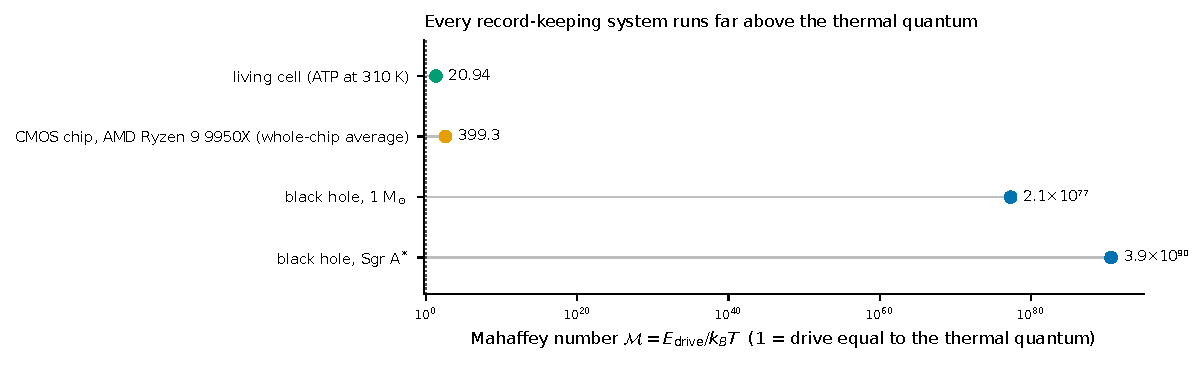
\includegraphics[width=\textwidth]{figures/part1/fig_mahaffey_number.pdf}
\caption{The Mahaffey number $\mathcal M=E_{\rm drive}/k_BT$ for the systems this book evaluates. Cell: one ATP, $54\,{\rm kJ\,mol^{-1}}$ at 310.15\,K, $\mathcal M=20.94$ (30.2 in Landauer units). Chip: whole-chip average $E_{\rm drive}={\rm TDP}/(Nf)$ at $T_j=75\,^\circ$C for 170\,W, $20.6\times10^9$ transistors, 4.3\,GHz (Chapters~\ref{ch:cmos} and \ref{ch:onegauge}, Part~\ref{part:5}; $\mathcal M=399$). Black holes: $Mc^2/k_BT_{\rm BH}=2S_{\rm BH}/k_B$, $2.1\times10^{77}$ for one solar mass and $3.9\times10^{90}$ for Sgr~A$^*$ ($4.3\times10^6\,M_\odot$). \calc}\label{fig:mahaffey_number}
\end{figure}
IAM's Law states that every irreversible quantum-to-classical transition pays $k_BT_H\ln2$ per bit to the nearest encoding surface. Dividing the energy
that drives irreversible information events in a system by the thermal quantum of its local encoding surface yields a dimensionless ratio that
characterizes the operating regime of the system,
\begin{equation}
\mathcal M=\frac{E_{\rm drive}}{k_BT_{\rm local}}, \label{eq:law_mahaffey}
\end{equation}
where $E_{\rm drive}$ is the energy source driving irreversible information events and $T_{\rm local}$ the temperature of the local encoding surface.
$\mathcal M$ is the Mahaffey number --- a dimensionless figure characterizing how far above the thermal floor a record-keeping system operates, following
the convention of Reynolds (fluid flow regimes), Mach (compressible flow), Froude (free-surface flow) and Prandtl (heat transfer) for dimensionless numbers
that characterize physical operating regimes. When $\mathcal M$ reaches an architecture-specific critical value, the local encoding surface saturates
and a phase transition occurs \conjecture. Expressed in Landauer units it is $\mathcal M/\ln2$. $\mathcal M$ is not a new law: it is IAM's Law,
Eq.~\eqref{eq:law}, expressed in dimensionless form. Landauer's principle taken alone is a floor with no structure: it does not say which temperature enters, where the record resides, or what
happens as a system approaches the bound. The law supplies the first two, the nearest encoding surface and its temperature; the third is the
saturation conjecture stated here, which Landauer's principle alone cannot make, because it has no surface and no capacity \interp. $\mathcal M$ is
dimensionless in every row and computed from measured quantities, so it is the part of the construction least dependent on anything contested \interp.
Every application of IAM's Law is a computation of $\mathcal M$ in domain-specific units:
\begin{itemize}
\item Thermal systems (semiconductor switching, superconducting qubit decoherence): $E_{\rm drive}=k_BT$, giving $\mathcal M=T/T_{\rm local}$.
Temperature is the lever. For a record held in a gap $hf$, $\mathcal M=hf/\kB T$ and the thermal floor of the record is $1/(1+e^{\mathcal M})$,
the same form as the cell's copy-error floor; one gate of duration $t_g$ is kicked out of its level with that occupation times $t_g/T_1$ (Chapter~\ref{ch:qplatforms}) \derived.
\item Chemical systems (living cells): $E_{\rm drive}=\Delta G_{\rm ATP}$, $T_{\rm local}=T_{\rm body}=310.15$\,K (fixed). $\mathcal M=\Delta G_{\rm ATP}/(RT_{\rm body})=20.94$
($30.2$ in Landauer units) \calc. Biology decoupled $E_{\rm drive}$ from $k_BT_{\rm local}$ by using chemical rather than thermal drive --- which is how it
keeps high-fidelity records at a fixed temperature far above the thermal floor \interp.
\item Cosmological (gravitational decoherence): $E_{\rm drive}$ is gravitational binding energy; $T_{\rm local}=T_H=\hbar H/(2\pi k_B)$. $\mathcal M$
integrated self-consistently over cosmic time with gravitational feedback is read as the activation function $E(a)=\exp(1-1/a)$: the activation
function is $\mathcal M$ solved with feedback \conjecture. Carrying out that integration is the next step.
\item Gravitational saturation (black holes): $E_{\rm drive}=Mc^2$, $T_{\rm local}=T_{\rm BH}=\hbar c^3/(8\pi GMk_B)$. Then
$\mathcal M=Mc^2/(k_BT_{\rm BH})=8\pi GM^2/(\hbar c)=2S_{\rm BH}/k_B$, the Smarr relation again~\cite{Smarr1973} \derived: gravity is simultaneously the drive
energy and the output of saturation.
\end{itemize}
With the architecture of the system, $\mathcal M$ sets the IAM floor (Chapter~\ref{ch:surfaces}).

The universal statement is: IAM's Law leaves a fingerprint across every physical domain. The fingerprint is $\mathcal M$. From the cosmic horizon to the
transistor junction to the human cell nucleus, every irreversible information event is a computation of the same ratio --- drive energy against the
thermal floor, normalized by the architecture of the local encoding surface \interp.

Measurement as a thermodynamic transaction is taken up in Part~\ref{part:qp} (Chapter~\ref{ch:measurement}); the interpretation, in Part~\ref{part:5}: the arrow of
time (Chapter~\ref{ch:time}) and the coincidence of dark energy with structure formation (Chapter~\ref{ch:theoryinterp}). The exponent $n=7/2$ rests on the
horizon accounting of Section~\ref{sec:law_exponent}; the halo count is its independent test.

The Mahaffey number is built from quantities already measured in cosmology, chip design and cell biology. Anyone working in one of those fields can compute it for their own system, in their own units, and check whether it behaves the way this chapter says. That is the most direct way to test IAM's Law, and the most direct way to break it.
